\section{Introduction}

--- STILL DRAFTING ---

Computational analysis has become an integral part of modern-day plant pathology. High-quality genome sequences are being generated for multiple plant and pathogen species including banana and \ac{Fo}. The \ac{ncbi} genome database currently holds 17 genome entries for the Musaceae family and 736 genome entries for \ac{Fo}, 17 of which are from \ac{Focub}, including a high-quality draft genome for \ac{Focub4} \parencite{Warmington2019} and \ac{Focub1} \parencite{Asai2019} (\href{https://www.ncbi.nlm.nih.gov/data-hub/genome/}{https://www.ncbi.nlm.nih.gov/data-hub/genome/} Accessed: 17/01/2024). Many bioinformatic tools have been developed to analyse the increasing number of genome sequences. For instance, \textcite{Park2010} highlight integrated platforms supporting strain identification, phylogenetics, comparative genomics, and knowledge sharing for \textit{Fusarium}. The use of genomics to identify \acf{ce} in \ac{Fo} is becoming commonplace and is contributing to our understanding of \ac{Fo} classification, evolution, and cryptic host specificity. 

Generally, fungal effectors do not share homology or conserved motifs, so computational prediction of fungal \acp{ce} is challenging \parencite{Sperschneider2022, Todd2022}. Broadly, fungal effectors have been predicted using a set of common characteristics: the presence of a secretion signal, sequence length $\leq$ 300 amino acids, and cysteine richness \parencite{Sperschneider2015}. Other features sometimes used to filter protein sets include the lack of a transmembrane domain; increased expression during host interaction; restricted taxonomic distribution without (or with minimal) sequence resemblance to other organisms; and encoded by genes featuring extended intergenic regions or located in gene-sparse, repeat-rich chromosomes \parencite{Dalio2018, Todd2022}. However, as \textcite{LoPresti2015, Sperschneider2015} stress, not all secreted proteins with small size and high cysteine content necessarily serve as effectors. Conversely, fungal effectors are not universally small and cysteine-rich. Larger proteins can also function as effectors, which leads \textcite{LoPresti2015} to describe the 300 amino acid cutoff as arbitrary. Further, effector classification often relies on the absence of detectable orthologous proteins beyond the genus, but some effectors may show conservation or possess conserved functional domains \parencite{Jonge2010, Djamei2011, Mentlak2012}. Given these uncertainties in effector definition, \textcite{LoPresti2015} adopt a broad perspective, considering any secreted fungal protein as a potential effector. 

\textcite{Sperschneider2016} developed a \ac{ml} tool, EffectorP v1.0, for the identification of effectors in fungi in an attempt to combat the challenges of effector discovery, explained by \textcite{Sperschneider2015, LoPresti2015}. EffectorP v1.0 is a Naïve Bayes \ac{ml} predictor, which was initially trained with 58 true fungal effectors from 16 species and achieved sensitivity and specificity of over 80\% \parencite{Sperschneider2016}. The negative dataset contained 14,143 proteins based on the total set of predicted secreted proteins from their 16 species (filtering the known effectors and homologs), and likely encompassed undiscovered effectors as well as non-effectors. Subsequently, EffectorP v2.0 was trained with 94 secreted true effectors from 23 species, utilising a refined negative dataset. This updated version successfully reduced effector candidates from fungal plant symbionts and saprophytes by 40\%, surpassing EffectorP v1.0 \parencite{Sperschneider2018}. EffectorP v2.0 has been employed by \textcite{Simbaqueba2020} in their analysis of \ac{Fo} f. sp. \textit{physalis}, identifying novel \acp{ce}. The latest iteration, EffectorP v3.0, introduces a classification based on apoplastic and cytoplasmic localisation \parencite{Sperschneider2022}. 

\Acp{mimp} provide an advantage when attempting to identify \acp{ce} in \ac{Fo} genomes, as they are found upstream of all known effectors in \ac{Foly} \parencite{Schmidt2013} (see: section \ref{Chap1:fusariumEffectorome}). \textcite{Dam2016} developed a computational pipeline (hereafter: FoEC) which identifies effectors using \acp{mimp} to reveal effector profiles of cucurbit-infecting \ac{Fo} strains. The FoEC pipeline first identifies \acp{mimp} in a \ac{Fo} genome by searching for the \ac{mimp} \acp{tir} through regular expression. Once \acp{mimp} have been identified, FoEC expands 2500bp downstream of the \ac{mimp} finding \acp{orf} using a custom Python script or using AUGUSTUS \parencite{Stanke2006} for gene prediction. Sequences are then filtered based on the presence or absence of a signal peptide, and redundancy, then searched against the input genome database using BLAST to create a presence/absence matrix. However, our analysis revealed that FoEC (v1) pipeline is unable to identify \acp{mimp} which have been soft-masked, a probable eventuality given that \acp{mimp} are repetitive elements. Removal of soft-masking to identify \acp{mimp} using FoEC (v1) will likely result in inaccurate gene predictions. Furthermore, FoEC (v1) only searches for effectors found downstream of a \ac{mimp}, but the study by \textcite{Schmidt2013} demonstrated that effectors may also be found upstream of a \ac{mimp}. 

FoEC has since been updated \parencite{FoEC2} (FoEC2)\footnote{Though it is not clear that the \ac{mimp} identification script has been adjusted to allow for soft-masking, it is of note that FoEC2 was developed and published following a discussion I had with the original FoEC authors.}, and uses a very similar pipeline structure. FoEC2 now also filters \acp{orf} based on cystine content and size (20aa $\leq$ size $\leq$ 600aa), clusters candidates using Diamond (v2.0.13) with Diamond BLASTP, MAFFT (v7.490) \parencite{Katoh2019} and uses HMMER \parencite{Eddy2011} to identify \acp{ce} in the original genome database. FoEC2 now contains some of the filtering criteria which, as explained by \textcite{Sperschneider2015, LoPresti2015, Todd2022}, can miss candidates. 

Though we recognise that FoEC2 can be used as a tool for the identification of \acp{ce} in \ac{Fo}, we developed a \ac{maei} pipeline\footnote{Development of the \ac{maei} pipeline was started before FoEC2 was published.} to find \acp{ce} in \ac{Fo} genomes and contribute to our understanding of virulence within the \ac{FOSC}. Our pipeline considers the concerns of \textcite{Sperschneider2015, Todd2022}, identifying small ($\leq$450aa), secreted proteins associated with \acp{mimp} (upstream and downstream, 2500bp) in the \ac{Fo} genomes, submitting them to EffectorP v2.0 for \ac{ce} prediction. We applied the \ac{maei} pipeline to investigate \ac{ce} profiles in \ac{r1} and \ac{tr4} \ac{Focub} genomes, as well as \ac{r1} and \ac{r4} genome assemblies of \ac{Fola}. \acp{ce} identified using the \ac{maei} tool can be used as a target for molecular diagnostics, which is currently being explored with \ac{r2}, \ac{r3}, and \ac{r4} isolates of \ac{Foa}. 

\newpage
\section{Materials and Methods}

\subsection{\textit{Fusarium} genome database generation}\label{chap3:fusariumdb}

\subsubsection{\textit{Fusarium} genome sequencing and assembly}

A database of both publicly available and new \textit{Fusarium} genome assemblies was produced for \ac{ce} identification and analysis (Table \ref{tab:GenomeDB})\footnote{The SY-2 isolate was included, but the S6, S16, and S32 genome assemblies were not included in this database as the raw read data were not available at the time.}. Collaborators at the \ac{niab} generated genome assemblies for \ac{Fo} \acp{fsp} \textit{lactucae} (\acs{Fola}) isolates AJ520, AJ718, AJ865, AJ516, AJ592, and AJ705; \textit{apii} (\acs{Foa}) isolates AJ498 and AJ720; \textit{coridandrii} (\acs{Foci}) isolate AJ615; \textit{matthiolae} (\acs{Foma}) isolate AJ260; \textit{narcissi} (\acs{Fona}) isolate FON63; and a \ac{Fo} isolate pathogenic towards rocket (\textit{Eruca vesicaria}), AJ174. These isolates were cultivated on \ac{pda} plates at 25°C for 4 days, and mycelial plugs were used to inoculate \ac{pdb} containing streptomycin. After 4 days of incubation, mycelium was harvested, lyophilised, and stored at -80°C. 

DNA extraction from 20mg of lyophilised mycelium was performed using a Macher\-ey-Nagel NucleoSpin Plant II kit (Fisher Scientific) with additional chloroform extraction after cell lysis. DNA samples were eluted in 30µl 10mM Tris HCl pH8 and analysed for quantity and purity using Nanodrop and Qubit (ratios 260/280 between 1.8-2.0, 260/230 between 2.0-2.2)  and for integrity using the Agilent TapeStation (TS 4150, Agilent Technologies). DNA samples (molecular weight >50kb) underwent Illumina PCR-free and \ac{ont} long-read sequencing. Illumina sequencing was conducted as described previously \parencite{Armitage2018}. \ac{ont} sequencing utilised the ligation sequencing kit (LSK108 for \ac{Foma} AJ260, \ac{Fona} FON63; or LSK110 all \ac{Fola}, \ac{Foa}, \ac{Foci} and \ac{Fo} rocket isolates) with flow cells FLO-MIN106 R9.4 (\ac{Foma} AJ260, \ac{Fona} FON63) or FLO-MIN106 R9.4.1 (\ac{Fola}, \ac{Foa}, \ac{Foci} and \ac{Fo} rocket isolates). 

Collaborators used \Ac{ont} long-read sequence data to construct \textit{de novo} genome assemblies. NanoPlot (v1.30.1) \parencite{DeCoster2018} was used for quality control of \ac{ont} data and Porechop (v0.2.4) (\href{https://github.com/rrwick/Porechop}{https://github.com/rrwic\-k/Porechop}), with default settings, was applied for adapter trimming. Filtlong (v0.2.1)  (\href{https://github.com/rrwick/Filtlong}{https://github.com/rrwick/Filtlong}) was used to remove reads shorter than 1 Kb or with a quality score less than Q9. Long-read data were assembled using NECAT (v0.0.1\_update20200803) \parencite{Chen2021} (genome size of 50 Mb) with parameters left as default. For long-read error correction, reads were aligned to the assemblies with Minimap2 (v2.17-r941) \parencite{Li2018} and used to inform one iteration of Racon v1.4.20 \parencite{Vaser2017}. This was followed by one iteration of Medaka (v1.5.0) (\href{https://github.com/nanoporetech/medaka}{https://github.com/nanoporetech/medaka}) using the r94\_min\_high\_g360 model. Illumina paired-end reads underwent quality control with FastQC (v0.11.9) (\href{https://www.bioinformatics.babraham.ac.uk/projects/fastqc/}{https://www.bioinformatics.babraham.ac.uk/projects/fastqc/}), followed by adapter and low-quality region trimming using Fastq-Mcf (v1.04) \parencite{Aronesty2013}. Alignment to long-read assemblies was conducted using Bowtie2 (v2.2.5) \parencite{Langmead2012} and SAMtools (v1.13) \Parencite{Danecek2021}. Three rounds of polishing with Pilon (v1.24) \parencite{Walker2014} corrected single base call errors and small insertions or deletions. Assembly statistics were computed using a custom Python script, and single copy ortholog analysis utilised \ac{busco} (v5.2.2) \parencite{Simao2015} with the hypocreales\_odb10 database.

\subsubsection{Publicly available \textit{Fusarium} genomes}

Two \ac{Fs} and 12 \ac{Focub} assemblies identified following GenBank genome search (\href{https://www.ncbi.nlm.nih.gov/data-hub/genome}{https://ww\-w.ncbi.nlm.nih.gov/data-hub/genome/}) were downloaded, as well as two \ac{Focub} genome assemblies (isolates 58 and 60) from the \ac{ngdc}, (\href{https://ngdc.cncb.ac.cn}{https:/\-/ngdc.cncb.ac.cn/}). Further, genome assemblies for the \ac{Foa} isolates AJ720 and AJ498 have already been published by \textcite{Henry2020} (AJ720 = 207.A, GCA\_014843455.1,  AJ498 = 274.AC, GCA\_014843565.1) so were used in this analysis for comparison. \Ac{Foa} \ac{r3} (NRRL38295, GCA\_014843565.1) and a \ac{Foci} (3-2, GCA\_014843415.1) genome assemblies generated by \textcite{Henry2020} were also included. A representative assembly (\( \leq \) 50 contigs and \(\geq \) 90\% complete BUSCOs reported) was included for other publicly available \textit{Fusarium} species and \acp{fsp}. As \textcite{Schmidt2013} reported no \acp{mimp} in the \ac{Fg} PH-1 genome, a reference assembly for \ac{Fg} PH-1 (GCA\_000240135.3) was included as an outgroup for phylogenies and negative control for \ac{mimp}-associated effector analysis.

\bigskip
\newcolumntype{C}[1]{>{\centering\arraybackslash}p{#1}}

\begingroup

\renewcommand{\arraystretch}{1}

\begin{ThreePartTable}
\footnotesize
\renewcommand\TPTminimum{\textwidth}
\setlength\LTleft{0pt}
\setlength\LTright{0pt}
\setlength\tabcolsep{0pt}

\begin{TableNotes}
    \item[a] Assemblies generated by collaborators at \ac{niab}. GenBank accession numbers are not currently available.
    \item[b] Assemblies generated in association with \ac{tnau}. GenBank accession numbers are not currently available.
    \item[c] Species not confirmed.
    \item[d] Included in RNA-seq analysis.
\end{TableNotes}

\begin{longtable}[c]{@{}C{2.5cm}C{0.8cm}C{2cm}C{2.8cm}C{1cm}C{1cm}C{1.5cm}C{0.7cm}C{2.5cm}@{}}
\captionsetup{width=\linewidth} 
\caption[Summary table of all \textit{Fusarium} assemblies included in effector analysis]{\textbf{Summary table of all \textit{Fusarium} assemblies included in effector analysis}. np= non-pathogen. Accessions shown are for GenBank (\href{https://www.ncbi.nlm.nih.gov/data-hub/genome}{\ac{ncbi} genome search}) or the \href{https://ngdc.cncb.ac.cn}{National Genomics Data Centre (NGDC)}, China.}

\label{tab:GenomeDB}\\
\toprule
\textbf{Species} &
  \textbf{Race} &
  \textbf{Isolate ID} &
  \textbf{Accession} &
  \textbf{Size (Mb)} &
  \textbf{Contig No.} &
  \textbf{Contig N50 (Mb)} &
  \textbf{GC (\%)} &
  \textbf{Completeness (\% complete BUSCOs)} \\* \midrule
\endhead
%
\bottomrule
\endfoot
%
\endlastfoot
%
\textit{F. graminearum}        &     & PH-1         & GCA\_000240135.3 & 38   & 5     & 9.3  & 48.2 &--    \\
\textit{Fo.} fsp. \textit{apii}         & 2   & AJ720\tnote{a}        &--             & 64.6 & 29    & 4.1  & 47.9 & 97.3 \\
\textit{Fo.} fsp. \textit{apii}         & 2   & 207.A        & GCA\_014843455.1 & 64.7 & 49    & 3.5  & 47.5 & 98.7 \\
\textit{Fo.} fsp. \textit{apii}         & 3   & NRRL38295    & GCA\_014843565.1 & 65.3 & 75    & 4    & 47.5 & 98.8 \\
\textit{Fo.} fsp. \textit{apii}         & 4   & AJ498\tnote{a}        & --             & 64.6 & 58    & 2.4  & 47.8 & 96.2 \\
\textit{Fo.} fsp. \textit{apii}         & 4   & 274.AC       & GCA\_014843565.1 & 67.3 & 114   & 4.4  & 47.5 & 98.8 \\
\textit{Fo.} fsp. \textit{capsici}      &     & Focpep1      & GCA\_016801315.1 & 54.5 & 34    & 5    & 47.5 & 93.5    \\
\textit{Fo.} fsp. \textit{cepae}        & 2   & FoC\_Fus2    & GCA\_003615085.1 & 53.4 & 34    & 4.1  & 47.5 & 99   \\
\textit{Fo.} fsp. \textit{conglutinans} &     & Fo5176       & GCA\_014154955.1 & 68   & 25    & 3.4  & 48   & 99.1 \\
\textit{Fo.} fsp. \textit{coriandrii}   &     & AJ615\tnote{a}        &--             & 69.3 & 45    & 3    & 48   & 97.5 \\
\textit{Fo.} fsp. \textit{coriandrii}   &     & 3-2          & GCA\_014843415.1 & 65.4 & 49    & 5    & 47.5 & 98.7 \\
\textit{Fo.} fsp. \textit{coriandrii}   &     & GL306        & GCA\_014843445.1 & 65   & 50    & 4.9  & 47.5 & 98.8 \\
\textit{Fo.} fsp. \textit{cubense}      & 1   & 160527       & GCA\_005930515.1 & 51.1 & 12    & 4.9  & 47   & 99.1 \\
\textit{Fo.} fsp. \textit{cubense}      & 1   & 60           & GWHAAST00000000  & 48.6 & 35    & 2.1  & 47.6 & 95.2 \\
\textit{Fo.} fsp. \textit{cubense}      & 1   & N2           & GCA\_000350345.1 & 47.7 & 2,185 & 0.1  & 48   &--    \\
\textit{Fo.} fsp. \textit{cubense}      & 4   & C1HIR\_9889  & GCA\_001696625.1 & 46.7 & 1,318 & 0.09 & 48.5 &--    \\
\textit{Fo.} fsp. \textit{cubense}      & 4   & B2           & GCA\_000350365.1 & 52.9 & 3,834 & 0.02 & 48   &--    \\
\textit{Fo.} fsp. \textit{cubense}      & TR4 & UK0001       & GCA\_007994515.1 & 48.6 & 15    & 4.5  & 47.5 & 98.4 \\
\textit{Fo.} fsp. \textit{cubense}      & TR4 & 58           & GWHAASU00000000  & 48.2 & 29    & 4.4  & 47.5 & 96.9 \\
\textit{Fo.} fsp. \textit{cubense}      & TR4 & Pers4        & GCA\_021237285.1 & 46.4 & 115   & 1.6  & 47.5 & 97.7 \\
\textit{Fo.} fsp. \textit{cubense}      & TR4 & II5\_54006   & GCA\_000260195.2 & 46.6 & 716   & 0.3  & 47.5 &--    \\
\textit{Fo.} fsp. \textit{cubense}      &     & VPRI44082    & GCA\_025216935.1 & 46.3 & 666   & 0.3  & 47   &--    \\
\textit{Fo.} fsp. \textit{cubense}      &     & VPRI44083    & GCA\_025216865.1 & 46.3 & 666   & 0.3  & 47   &--    \\
\textit{Fo.} fsp. \textit{cubense}      &     & VPRI44081    & GCA\_025216985.1 & 47.2 & 902   & 0.4  & 47   &--    \\
\textit{Fo.} fsp. \textit{cubense}      &     & VPRI44079    & GCA\_025216905.1 & 49.5 & 1801  & 0.3  & 47.5 &--    \\
\textit{Fo.} fsp. \textit{cubense}      &     & VPRI44084    & GCA\_025216845.1 & 50.2 & 2,807 & 0.3  & 47.5 &--    \\
\textit{Fo.} endophyte         & np  & Fo47\tnote{d}         & GCA\_013085055.1 & 50.4 & 12    & 4.5  & 47.5 & 99   \\
\textit{Fo.} fsp. \textit{lactucae}     & 1   & AJ865\tnote{a}        &--             & 62.7 & 38    & 2.7  & 47.7 & 95.3 \\
\textit{Fo.} fsp. \textit{lactucae}     & 1   & AJ718\tnote{a}        &--             & 62.1 & 39    & 2.5  & 47.6 & 95.6 \\
\textit{Fo.} fsp. \textit{lactucae}     & 1   & AJ520\tnote{a,d}        &--             & 62.2 & 40    & 2.9  & 47.6 & 95.1 \\
\textit{Fo.} fsp. \textit{lactucae}     & 4   & AJ705\tnote{a,d}        &--             & 66.2 & 32    & 3    & 47.7 & 97.7 \\
\textit{Fo.} fsp. \textit{lactucae}     & 4   & AJ592\tnote{a}        &--             & 66   & 36    & 2.6  & 47.7 & 97.5 \\
\textit{Fo.} fsp. \textit{lactucae}     & 4   & AJ516\tnote{a,d}        &--             & 68.8 & 37    & 3    & 47.6 & 97.6 \\
\textit{Fo.} fsp. \textit{lini}         &     & 39           & GCA\_012026625.1 & 59.2 & 34    & 3.4  & 47.5 & 99.5 \\
\textit{Fo.} fsp. \textit{lycopersici}  & 2   & 4287         & GCA\_001703175.2 & 56.2 & 47    & 4.1  & 47.5 & 99.5 \\
\textit{Fo.} fsp. \textit{matthiolae}   &     & AJ260\tnote{d}        & GCA\_020796175.1 & 60.3 & 40    & 4.5  & 47.5 & 97.8 \\
\textit{Fo.} fsp. \textit{matthiolae}   &     & PHW726\_1    & GCA\_009755825.1 & 57.2 & 585   & 0.7  & 47   &--    \\
\textit{Fo.} fsp. \textit{narcissi}     &     & FON63\tnote{a}        &--             & 60   & 34    & 4    & 47.9 &--    \\
\textit{Fo.} fsp. \textit{niveum}       & np  & 110407-3-1-1 & GCA\_019593455.1 & 49.7 & 33    & 2.8  & 47   & 99.8 \\
\textit{Fo.} fsp. \textit{rapae}        &     & Tf1208       & GCA\_019157295.1 & 59.8 & 25    & 4.2  & 47.5 & 99   \\
\textit{Fo.} from rocket      &     & AJ174\tnote{a}        &--             & 62.6 & 30    & 2.7  & 47.9 & 97.8 \\
\textit{Fo.} fsp. \textit{vasinfectum}  & 1   & TF1          & GCA\_009602505.1 & 50   & 17    & 4.2  & 47   & 98.8 \\
\textit{F. sacchari}           & 1   & FS66         & GCA\_017165645.1 & 47.5 & 47    & 2    & 48   & 99.5 \\
\textit{F. sacchari}           &     & NRRL 66326   & GCA\_013759005.1 & 42.8 & 515   & 0.2  & 49   &--    \\
\textit{Fusarium}\tnote{c}              &     & SY-2\tnote{b}         &--             & 46.3 & 441   & 0.2  & 46.6 & 99.6 \\* \bottomrule
\insertTableNotes
\end{longtable}
\end{ThreePartTable}
\endgroup
\bigskip

\newpage

\subsection{Phylogenetic analysis of \textit{Fusairum} isolates}

\Ac{tef} and \ac{rbp2} phylogenies were generated as previosuly described (section:~\ref{chap2:phylogeny}) for the \textit{Fusarium} assemblies included in the \ac{ce} analysis. Briefly, homologues of each \ac{tef} and \ac{rbp2} were identified in each assembly in our database  (Table \ref{tab:GenomeDB}) using BLASTN (1e-\textsuperscript{6} cut-off). The locations of hits with greater than 70\% identity and 90\% coverage were extracted using SAMtools (v1.15.1). \Ac{tef} and \ac{rbp2} sequences from each genome were concatenated into a single FASTA file for each barcode and aligned using MAFFT (v7.505) \parencite{Katoh2019}. IQ-TREE (v2.2.0.3) \parencite{Nguyen2015} was used to infer a maximum-likelihood phylogeny using the ultrafast bootstrap setting for 1000 bootstrap replicates and was visualised using the R \parencite{R} (v4.3.1), ggtree (v3.10.0) \parencite{ggtree}.



%\subsection{Identification of \textit{SIX} genes in \textit{Fusarium oxysporum} genome assemblies}

%As described previously (section: \ref{chap1:tnauSIXgenePhylo}), the complement of \ac{sixg} homologues was determined in all the \ac{Fo} genomes generated in this study, as well as in publicly available genomes (Table \ref{tab:GenomeDB}). \Ac{sixg} phylogenies were  constructed for the \acp{sixg} present in \ac{Fola} \ac{r1} (SIX9, SIX14) and \ac{Fola} \ac{r4} (SIX8, SIX9, SIX14). 

\subsection{\textit{Mimp}-associated effector identification (Maei) pipeline}

\subsubsection{\Ac{mimp} identification}

A \acf{maei} pipeline for the identification of \acp{ce} in \ac{Fo} was developed (Figure: \ref{fig:MaeiPipeline}). The \ac{maei} pipeline first identifies \acp{mimp} in \textit{Fusrium} genomes. Two methods of \textit{mimp} searching were developed. The first identifies \acp{mimp} using a custom Python (v3.8.8) script \parencite{Python} which uses the Biopython (v1.78) package \parencite{biopython}. As performed in \textcite{Schmidt2013, Dam2016, Armitage2018} \acp{mimp} were identified in each \textit{Fusarium} genome using regular expression, whereby the \textit{mimp1-4} consensus \ac{tir} sequences \parencite{Bergemann2008, Schmidt2013}, "CAGTGGG..GCAA[TA]AA" and "TT[TA]TTGC..CCCACTG", were used as a search pattern. Where sequences matching this pattern occured within 400 nucleotides of each other a \ac{mimp} was recorded (script available via \href{https://github.com/JamiePike/Maei/blob/main/bin/Mimp_finditer.py}{GitHub}). The second method employs a \acf{hmm} which was developed using the \ac{hmm} tool HMMER (v3.3.1) \parencite{Eddy2011}. Publicly available \ac{mimp} sequences (Appendix \ref{apx:RefMimps}) and \ac{mimp} sequences identified using the regular expression method were used to build a \ac{mimp} profile-\ac{hmm}. This profile-\ac{hmm} was used as the input for an NHMMER (v3.3.1) \parencite{Eddy2011} search of each genome (full command-line arguments available via GitHub: \href{https://github.com/JamiePike/Maei/blob/main/dev/notes/Mimp_Searching_Methods.md}{https://github.com/JamiePike/Maei/dev/notes/Mimp\_Searching\_Methods.md}).

\subsubsection{Sequence extraction}

Using \acp{mimp} identified by both \ac{mimp} searching methods, sequences 2.5kb upstream and downstream of each \ac{mimp} were extracted, merged (to create a non-redundant set), and stored in GFF3 format using the BEDtools (v2.25.0) suite \parencite{Quinlan2010} (full command-line arguments available on GitHub: \href{https://github.com/JamiePike/Maei/blob/main/bin/Maei_v5.sh}{https://github.com/JamiePike/Maei/bl\-ob/main/bin/Maei\_v5.sh}). Using the GFF3 locations, two FASTA files were generated i) "\ac{mimp}-region" FASTA where all nucleotides not within a 5kb window (2.5kb upstream + 2.5kb downstream) of a \ac{mimp} were hard-masked, ii) "AUGUSTUS-region" where all nucleotides outside of a 45kb window (22.5kb upstream + 22.5kb downstream) of a \ac{mimp} were hard-masked. The "AUGUSTS-region" FASTA file was generated with a 45kb window to prevent truncation of gene models. 

\Acp{orf} withing the "\ac{mimp}-regions" were identified using the EMBOSS (6.6.0.0) tool, getorf (https://www.bioinformatics.nl/cgi-bin/emboss/getorf). The "AUGUSTUS-region" FASTA was subjected to gene prediction using AUGUSTUS (3.3.3) \parencite{Stanke2006} with the “Fusarium” option enabled. The AUGUSTUS (v3.3.3) gene models and "\ac{mimp}-region" GFF3 files were intersected and merged using the BEDtools (v2.25.0) suite \parencite{Quinlan2010} to ensure that gene models which may be partially within the 5kb "\ac{mimp}-region" window are not truncated, but that gene models outside of the 5kb "\ac{mimp}-region" window but within the 45kb "AUGUSTUS-region" window are not included. The intersected AUGUSTUS (v3.3.3) gene models and "\ac{mimp}-region" GFF3 file was used as input for AGAT (v1.0.0) \parencite{DainatN.D.}, which was used extract AUGUSTUS (v.3.3.3) \ac{mimp}-associated gene models in FASTA file format. The \ac{mimp}-associated gene model FASTA file and getORF FASTA were merged to generate a \ac{mimp}-associated gene model and \ac{orf} FASTA file. The output from getORF was also converted to GFF3 format using a custom Python script (available via \href{https://github.com/JamiePike/Maei/blob/main/bin/getORF2bed.py}{ GitHub https://github.com/JamiePike/Maei/blob/main/bi\-n/getORF2bed.py}
). These GFFS were then merged to generate a \ac{mimp}-associated gene models and \acp{orf} GFF3 and FASTA file for each genome using BEDtools (v2.25.0) suite.

\subsubsection{\ac{ce} filtering and prediction}

Sequences from the \ac{mimp}-associated gene model and ORF FASTA were then filtered based on size using SAMtools (v1.6) and the BEDtools (v2.25.0) suite, with sequences >30aa and <450aa submitted to SignalP (v5.0b) \parencite{Petersen2011}. Sequences that were predicted to contain a signal peptide were passed to EffectorP (v2.0.1) \parencite{Sperschneider2018} for \ac{ce} prediction. This output is was to generate genome-specific, \ac{mimpce} sets.

\subsubsection{\Acl{cec}ing and distribution}

The genome-specific \ac{mimpce} sets were then combined and clustered using CD-HIT (v4.8.1) \parencite{Fu2012} at 80\% identity to generate \acfp{cec}. Data from CD-HIT (v4.8.1) was also passed to a custom Python script, which was used to generate an overview table and a distribution matrix (available via GitHub: \href{https://github.com/JamiePike/Maei/blob/main/bin/Processingcdhit.py}{https://github.com/Jamie\-Pike/Maei/blob/main/bin/Processingcdhit.py}).

To identify candidates which may be shared across isolates but not associated with a \ac{mimp} in all isolates, the combined genome-specific \ac{mimpce} sets were then searched against the \textit{Fusarium} genomes using TBLASTN, with a cut-off 1e-6 and a percentage identity and coverage threshold of 65\%. Sequences within the threshold were extracted using  SAMtools (v1.6) and the BEDtools (v2.25.0) suite and were subjected to filtering using SignalP (v5.0b), default settings and EffectorP (v2.0.1) to remove unlikely candidates. The remaining sequences (hereafter: \acf{ce}s) were clustered using CD-HIT (v4.8.1) \parencite{Fu2012} at 65\% identity to generated \acp{cec}. To identify differences in the distribution of \acp{cec} among assemblies, a binary presence/absence matrix was generated, where presence ("1") for a given isolate was counted if $\geq1 $ \ac{ce} clustered within a \ac{cec}.

Pearsons’s correlation was performed in R (v4.3.1) \parencite{R} to investigate the relationship  between genome size, \ac{mimp} and \ac{ce} content. The distribution of \acp{cec} across \textit{Fusarium} genomes assemblies was recorded in a binary matrix and hierarchical clustering of \acp{cec} distribution was performed using the R (v4.3.1) \parencite{R} package, ComplexHeatmap (v2.15.4)  \parencite{ComplexHeatmap} setting the clustering distance for rows and columns to "binary". Additional \ac{cec} distribution heatmaps and \ac{tef} phylogenies were generated for \ac{Focub}, \ac{Foci} and \ac{Foa}, as well as \ac{Fola} using the R (v4.3.1) package ggtreeExtra (v1.13.0) \parencite{ggtree}. The full R script is available in Markdown format in the GitHub repository associated with the project (\href{https://github.com/JamiePike/Maei/blob/main/exp/AllFusAnalysis-Chap3/R/AnalysisCandidateEffectorSets.md}{https://github.com/JamiePike/Maei/blob/main/exp/AllFusAnalysis-Chap3/R/Ana\-lysisCandidateEffectorSets.md}) 

\begin{figure}[htp!]
    \centering
    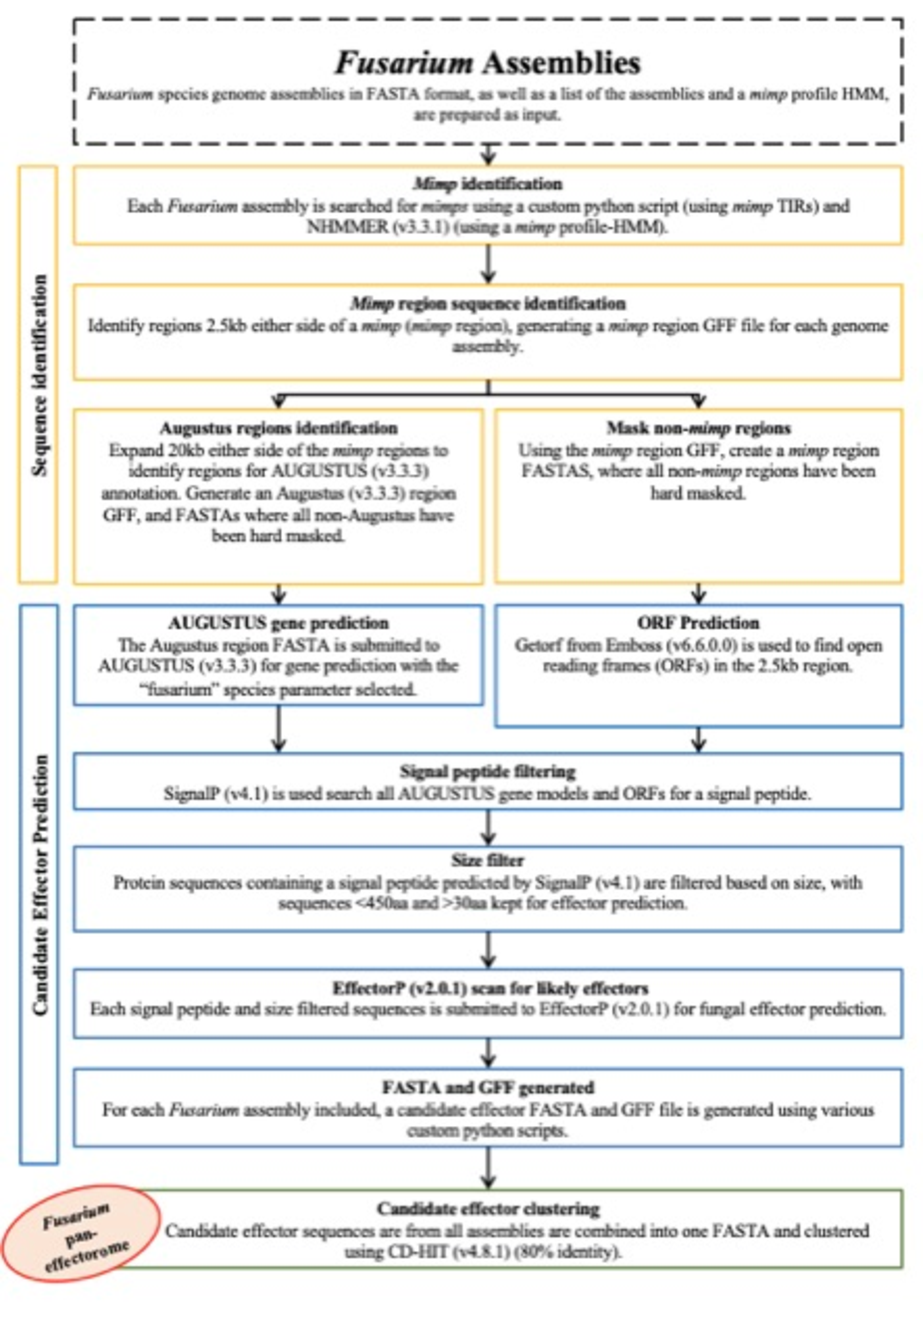
\includegraphics[width=14cm]{Figures/Maie_v5_Figure-portrait.pdf}
    \caption[Overview of the \acf{maei} pipeline.]{\textbf{Overview of the \acf{maei} pipeline.}}  
    \label{fig:MaeiPipeline}
\end{figure}

\subsection{Identification of reciprocal best hits \acl{tnau} \aclp{ce} against \textit{Fusarium} of banana pathogens}

The MMseq2 easy-rbh (v13.45111) \parencite{Steinegger2017} was used to identify reciprocal best hits of \acp{ce} identified in the \ac{tnau} genome assemblies for isolates, S6, S16, S32, and SY-2, against \ac{ce} sets identified as part of the \ac{maei} pipeline from \textit{Fusarium} pathogenic towards banana. Default easy-rbh settings were used. Full command line arguments can be found in the associated documents of the \ac{maei} GitHub repository (\href{https://github.com/JamiePike/Maei}{https://github.com/JamiePike/Maei}).   

\subsection{Identification and phylogenetic analysis of \aclp{sixg} in \acl{Fola}}

The set of homologues for SIX genes (\acp{sixg}) was determined in all genomes of \ac{Fola} and other \textit{F. oxysporum} isolates, produced in collaboration with \ac{niab}, as well as in publicly available genomes for the \textit{F. oxysporum} endophyte Fo47, and for \ac{Fo} \acp{fsp} \textit{capsici, cepae, conglutinans, coriandrii, cubense, lini, luffae, lycopersici, matthiolae, niveum, rapae}, and \textit{vasinfectum} obtained from GenBank through a genome search (\url{https://www.ncbi.nlm.nih.gov/data-hub/genome/}) \textcolor{red}{(Appendix SD1-T2)}. Reference sequences for SIX1-SIX15 from \ac{Foly} (isolate 4287) were retrieved from the NCBI database \textcolor{red}{(Supplementary data SD1-T4)}, and homologues of each \ac{sixg} were identified in each assembly using tBLASTx (1e-\textsuperscript{6} cut-off). A binary data matrix indicating presence (“+”) or absence (“-”) was generated based on the tBLASTx hit data. Phylogenies for \acp{sixg} were then constructed for the \acp{sixg} present in \ac{Fola} \ac{r1} (\textit{SIX9, SIX14}) and \ac{Fola} \ac{r4} (\textit{SIX8, SIX9, SIX14}). The positions of tBLASTx hits for \textit{SIX8}, \textit{SIX9}, and \textit{SIX14} were recorded (1e-\textsuperscript{6} cut-off), and the sequence within these regions was extracted using SAMtools (v1.15.1). Extracted regions from each genome were concatenated into a single FASTA file for each \ac{sixg}. Multiple sequence alignment was performed using MAFFT (v7.505) \parencite{Katoh2019}, with the “—adjustdirectionaccurately” and “–reorder” options. To ensure accurate alignment, any overhanging regions were manually inspected and trimmed. Maximum-likelihood phylogenies were inferred using IQ-TREE (v2.2.0.3) \parencite{Nguyen2015} with the ultrafast bootstrap setting for 1000 bootstrap replicates, and the resulting trees were visualised using iTOL \parencite{Letunic2021}.


\subsection{Expression and putative function of \acp{ce}}

\subsubsection{\Acf{Fola} inoculation, RNA extraction and RNAseq analysis}

Collaborators at \ac{niab} inoculated lettuce seedlings with \ac{Fola} and non-pathogenic \ac{Fo} isolates and conducted RNA extraction and analysis. Their method was adapted from \textcite{Taylor2016}. Two variants of Fola4 (AJ516, AJ705) and Fola1 AJ520 were used, along with controls: Foma AJ260 (pathogenic on column stocks) and F. oxysporum Fo47 (non-pathogenic isolate) (isolates indicated in table \ref{tab:GenomeDB}). A non-inoculated control treatment was also established. Autoclaved ATS medium (1 M KNO\textsubscript{3}, 1 M KPO\textsubscript{4}, 1 M MgSO\textsubscript{4}, 1 M Ca(NO\textsubscript{3})\textsuperscript{2}, 20 mM Fe-EDTA, 70 mM H\textsubscript{3}BO\textsubscript{3}, 14 mM MnCl\textsubscript{2}, 0.5 mM CuSO\textsubscript{4}, 1 mM ZnSO\textsubscript{4}, 0.2 mM Na\textsubscript{2}MoO\textsubscript{4}, 10 mM NaCl, 0.01 mM CoCl\textsubscript{2}, 0.45\% Gelrite) (Duchefa Biochemie, Haarlem, The Netherlands) in square petri dishes (12 x 12 x 1.7 cm, Greiner Bio-One, UK) was used for growth. \ac{Fola}-susceptible lettuce seeds (cv. Kordaat) were surface-sterilised (10\% bleach water (v/v) solution for 5 min and then rinsed three times with \ac{sdw}) and placed on agar plates. Stacks of plates were chilled for 4 days, followed by incubation at 15°C for 8 days and then 25°C for six days. Conidial suspensions of each two-week old \ac{Fo} culture (grown on \ac{pda} at 25°C) was prepared, adjusted to 1 x 10\textsuperscript{6} spores mL\textsubscript{-1} in \ac{sdw} with the addition of 200 \(\mu\)L of Tween20 L\textsubscript{-1}, and 1.5mL pipetted directly onto lettuce roots (seven agar plates per isolate). Non-inoculated controls received \ac{sdw} + Tween. RNAseq samples were obtained from lettuce roots at 96 \ac{hpi} (four agar plates per isolate) and pooled in to one sample of 12 plants per plate, corresponding to the peak expression of \textit{SIX8}, \textit{SIX9}, and \textit{SIX14} (data not shown). Lettuce roots were rinsed in \ac{sdw}, flash frozen in liquid nitrogen and stored at -80°C before extraction. Disease assessment was conducted two \ac{wpi} (using three remaining plates per isolate).

In order to identify unregulated genes \textit{in planta}, \ac{Fo} isolates were cultured \textit{in vitro}. Spore suspensions (500 \(\mu\)L 1 x 10\textsuperscript{6} spores mL\textsubscript{-1}) were pipetted onto \ac{pda} plates (prepared as above) with autoclaved cellulose discs and incubated for 96 hours at 25°C. Mycelium was harvested by scraping off the layer growing on the cellulose surface followed by flash freezing. 

Lettuce roots were ground to a fine powder using a pestle and mortar filled with liquid nitrogen and approximately 100 mg of tissue transferred to a 2 mL tube. RNA was extracted using Trizol® reagent (Thermo Fisher Scientific). Extracted RNA was precipitated using \(\mu\)L of lithium chloride to 100 \(\mu\)L of RNA (250 μL LiCl2 + 650 μL DEPC treated water). DNase1 (Sigma-Aldrich) was used to remove DNA. To check degredation, RNA samples were visualised on a 2\% agarose gel (containing GelRedTM at 2 μL per 100 mL of gel) with Orange G (Sigma-Aldrich) loading dye. RNA samples were sent to  Novogene conducted polyA-enrichment, followed by Illumina PE150 sequencing at a depth of 23G raw data per sample for \textit{in planta} samples and 9G per sample for \textit{in vitro} mycelial RNA samples.

Transcripts from both \ac{Fo} isolates and lettuce RNA-Seq reads had  adaptees trimmed using Fastq-Mcf (v1.04) \parencite{Aronesty2013}. To distinguish \ac{Fo} reads from lettuce, the lettuce genome (\textit{Lactuca sativa}, \ac{ncbi} accession: GCF\_002870075.3) was obtained from \ac{ncbi}. Pre-processed reads were then aligned to respective F. oxysporum assemblies using \ac{star} (v2.7.10) \parencite{Dobin2013}, incorporating the flag --outReadsUnmapped to generate a file containing non-mapping reads. The non-mapping putative \ac{Fo} RNA-Seq reads were pseudo-aligned to the respective reference genome and quantified using Kallisto (v0.48.0) \parencite{Bray2016}. Subsequently, R (v4.1.3) \parencite{R} and the DESeq2 package (v1.34.0) \parencite{Love2014} were utilised for conducting differential gene expression analysis. The contrast function was applied to produce a list of deferentially expressed genes.

\subsubsection{\textcolor{red}{Functional predictions}}

\subsection{Data and software availability}

The complete computational pipelines, along with command-line arguments and bash, R, and Python scripts employed for the \ac{cec} identification and analyses, can be accessed in the Maei GitHub Repository (\href{https://github.com/JamiePike/Maei}{https://github.com/JamiePike/Maei}). Previous versions and supporting development documentation is available in Markdown format for \ac{maei} \href{https://github.com/JamiePike/Maei/tree/main/dev}{pipeline development}.

\newpage
\section{Results}

\subsection{Relationship between \acp{mimp}, \acp{ce} and genome assembly size}

\Acp{mimp} and \acfp{ce} were identified in all 42 genome assemblies included in the \ac{maei} analysis. The number of \acp{mimp} ranged from one in the \ac{Fg} PH-1 assembly to 675 in the assembly for \ac{Foci} AJ615, with an average of 277 identified across all genome assemblies (Table \ref{tab:CandEffNo}). \Acp{ce} showed a comparable range, with only six identified in the \ac{Fg} PH-1 assembly and 603 identified in \ac{Foci} AJ615, averaging 206 per assembly. Assemblies with more \acp{mimp} tended to have higher counts of \acp{ce}. Pearson's correlation analysis revealed a strong positive relationship between \acp{mimp} and \acp{ce} (r(40) = 0.88, p < 0.01). 

\bigskip

\begingroup
\setlength{\tabcolsep}{6.1pt} % Default value: 6pt
\renewcommand{\arraystretch}{0.62}
\setlength\LTcapwidth{\textwidth} % default: 4in (rather less than \textwidth...)
\setlength\LTleft{0pt}            % default: \parindent
\setlength\LTright{0pt} % default: \fill
\footnotesize
\begin{longtable}{@{}lcccccc@{}}
\caption[Number of \acp{mimp}, \aclp{ce}, and \aclp{cec} identified in \textit{Fusarium} genomes.]{\textbf{Number of \acfp{mimp}, \acfp{ce}, and \acfp{cec} identified in \textit{Fusarium} genomes.} np indicates non-pathogen.}
\label{tab:CandEffNo}\\
\toprule
\textbf{Species} & \textbf{\acl{fsp}} & \textbf{Race} & \textbf{Isolate} & \textbf{No. \acp{mimp}} & \textbf{No. \acp{ce}} & \textbf{No. \acp{cec}} \\* \midrule
\endhead
%
\bottomrule
\endfoot
%
\endlastfoot
%
\textit{F. oxysporum} & \textit{apii} & Race 2 & 207A & 420 & 388 & 103 \\
\textit{F. oxysporum} & \textit{apii} & Race 2 & AJ720 & 442 & 399 & 101 \\
\textit{F. oxysporum} & \textit{apii} & Race 3 & NRRL38295 & 210 & 328 & 87 \\
\textit{F. oxysporum} & \textit{apii} & Race 4 & 274AC & 217 & 357 & 90 \\
\textit{F. oxysporum} & \textit{apii} & Race 4 & AJ498 & 539 & 332 & 90 \\
\textit{F. oxysporum} & \textit{cepae} & Race 2 & FoC\_Fus2 & 325 & 359 & 84 \\
\textit{F. oxysporum} & \textit{conglutins} &  & Fo5176 & 442 & 385 & 87 \\
\textit{F. oxysporum} & \textit{coriandrii} &  & 3-2 & 478 & 315 & 99 \\
\textit{F. oxysporum} & \textit{coriandrii} &  & AJ615 & 675 & 603 & 106 \\
\textit{F. oxysporum} & \textit{cubense} & Race 1 & 160527 & 183 & 95 & 49 \\
\textit{F. oxysporum} & \textit{cubense} & Race 1 & 60 & 39 & 45 & 34 \\
\textit{F. oxysporum} & \textit{cubense} & Race 1 & N2 & 141 & 63 & 42 \\
\textit{F. oxysporum} & \textit{cubense} & Tropical Race 4 & 58 & 165 & 108 & 45 \\
\textit{F. oxysporum} & \textit{cubense} & Tropical Race 4 & B2 & 142 & 60 & 42 \\
\textit{F. oxysporum} & \textit{cubense} & Tropical Race 4 & C1HIR\_9889 & 145 & 70 & 43 \\
\textit{F. oxysporum} & \textit{cubense} & Tropical Race 4 & NRRL\_54006 & 105 & 70 & 43 \\
\textit{F. oxysporum} & \textit{cubense} & Tropical Race 4 & Pers4 & 87 & 62 & 45 \\
\textit{F. oxysporum} & \textit{cubense} & Tropical Race 4 & UK0001 & 160 & 127 & 46 \\
\textit{F. oxysporum} & \textit{cubense} &  & VPRI44079 & 149 & 107 & 53 \\
\textit{F. oxysporum} & \textit{cubense} &  & VPRI44081 & 137 & 45 & 40 \\
\textit{F. oxysporum} & \textit{cubense} &  & VPRI44082 & 146 & 50 & 47 \\
\textit{F. oxysporum} & \textit{cubense} &  & VPRI44083 & 146 & 50 & 47 \\
\textit{F. oxysporum} & \textit{cubense} &  & VPRI44084 & 179 & 104 & 56 \\
\textit{F. oxysporum} & endophyte & np & Fo47 & 70 & 81 & 53 \\
\textit{F. oxysporum} & from rocket &  & AJ174 & 419 & 169 & 78 \\
\textit{F. oxysporum} & \textit{lactucae} & Race 1 & AJ718 & 536 & 260 & 76 \\
\textit{F. oxysporum} & \textit{lactucae} & Race 1 & AJ865 & 569 & 296 & 76 \\
\textit{F. oxysporum} & \textit{lactucae} & Race 1 & AJ520 & 533 & 343 & 86 \\
\textit{F. oxysporum} & \textit{lactucae} & Race 4 & AJ592 & 615 & 482 & 85 \\
\textit{F. oxysporum} & \textit{lactucae} & Race 4 & AJ705 & 614 & 490 & 83 \\
\textit{F. oxysporum} & \textit{lactucae} & Race 4 & AJ516 & 522 & 548 & 90 \\
\textit{F. oxysporum} & \textit{lini} &  & 39\_C0058 & 263 & 237 & 87 \\
\textit{F. oxysporum} & \textit{lycopersici} & Race 2 & 4287 & 332 & 337 & 80 \\
\textit{F. oxysporum} & \textit{matthiolae} &  & AJ260 & 301 & 209 & 76 \\
\textit{F. oxysporum} & \textit{narcissus} &  & FON63 & 555 & 251 & 91 \\
\textit{F. oxysporum} & \textit{niveum} & np & 110407-3-1-1 & 52 & 39 & 36 \\
\textit{F. oxysporum} & \textit{rapae} &  & Tf1208 & 377 & 278 & 82 \\
\textit{F. oxysporum} & \textit{vasinfectum} & Race 1 & TF1 & 199 & 91 & 58 \\
\textit{F. graminearum} &  &  & PH-1 & 1 & 6 & 5 \\
\textit{F. sacchari} &  &  & FS66 & 9 & 12 & 12 \\
\textit{F. sacchari} &  &  & NRRL\_66326 & 10 & 15 & 15 \\
\textit{Fusarium} &  &  & SY-2 & 3 & 12 & 12 \\* \bottomrule
\end{longtable}

\endgroup

To explore the distribution of \acp{ce} within \acp{fsp}, the \ac{maei} analysis incorporated multiple assemblies of \ac{Focub} (n=14), \ac{Fola} (n=6), \ac{Foa} (n=5), and \ac{Foci} (n=2). In \ac{Focub}, the average count of \acp{mimp} was 137, while the average count of \acp{ce} was 77. \ac{Foci} exhibited higher averages, with 577 \acp{mimp} and 459 \acp{ce}. \ac{Fola} and \ac{Foa} displayed intermediate values, with \ac{Fola} averaging 565 \acp{mimp} and 403 \acp{ce}, and \ac{Foa} 366 \acp{mimp} and 361 \acp{ce}. Notably, the larger genome assemblies tended to have higher \ac{mimp} and \ac{ce} counts. Pearson's correlation revealed that there was a significant positive correlation between genome assembly size and \ac{mimp} content (r(40) = 0.87, p < 0.01) and between genome assembly size and \ac{ce} content (r(40) = 0.91, p < 0.01) (Figure \ref{fig:MaeiStats}). 

\begin{figure}[ht!]
    \centering
    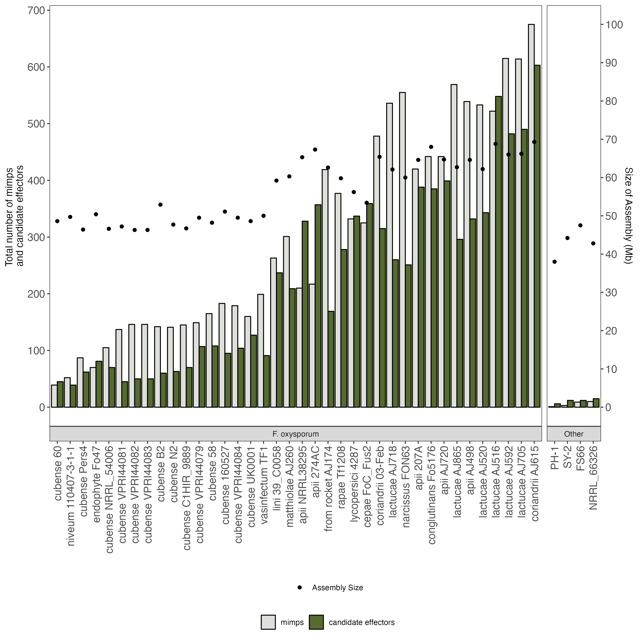
\includegraphics[width=\textwidth]{Figures/StatsOverview.png}
    \caption[Overview of \ac{ce} and \ac{mimp} content in relation to genome assembly size.]{\textbf{Overview of \ac{ce} and \ac{mimp} content in relation to genome assembly size.} A strong positive correlation between \ac{mimp} and \ac{ce} content (r(40)=0.88, p\textless0.01) was observed. Additionally, there is a significant positive correlation between genome assembly size and \ac{ce} content (r(40)=0.91, p\textless0.01), and between genome assembly size and \ac{mimp} content (r(40)=0.87, p\textless0.01).}
    \label{fig:MaeiStats}
\end{figure}

The average number of \acp{mimp} and \acp{ce} in different races of the same \ac{fsp} was also investigated. For the \ac{Fola} genome assemblies, the average number of \acp{mimp} was comparable, standing at 546 for \ac{r1} (n=3) and 583 for \ac{r4} (n=3). However, there was a notable disparity in the average counts of \acp{ce}, with 300 identified in the \ac{Fola} \ac{r1} genome assemblies (range: 260 to 343), compared to an average of 507 in the \ac{r4} assemblies (range: 482 to 548) (Figure \ref{fig:MaeiBoxPlot}). In \ac{Focub}, the difference in the number of  \acp{mimp} and \acp{ce} between races was less pronounced, with averages of 121 and 134 \acp{mimp}, and 68 and 83 \acp{ce} identified in the \ac{r1} (n=3) and \ac{tr4} (n=6) genome assemblies, respectively.

\bigskip
\begin{figure}[ht!]
    \centering
    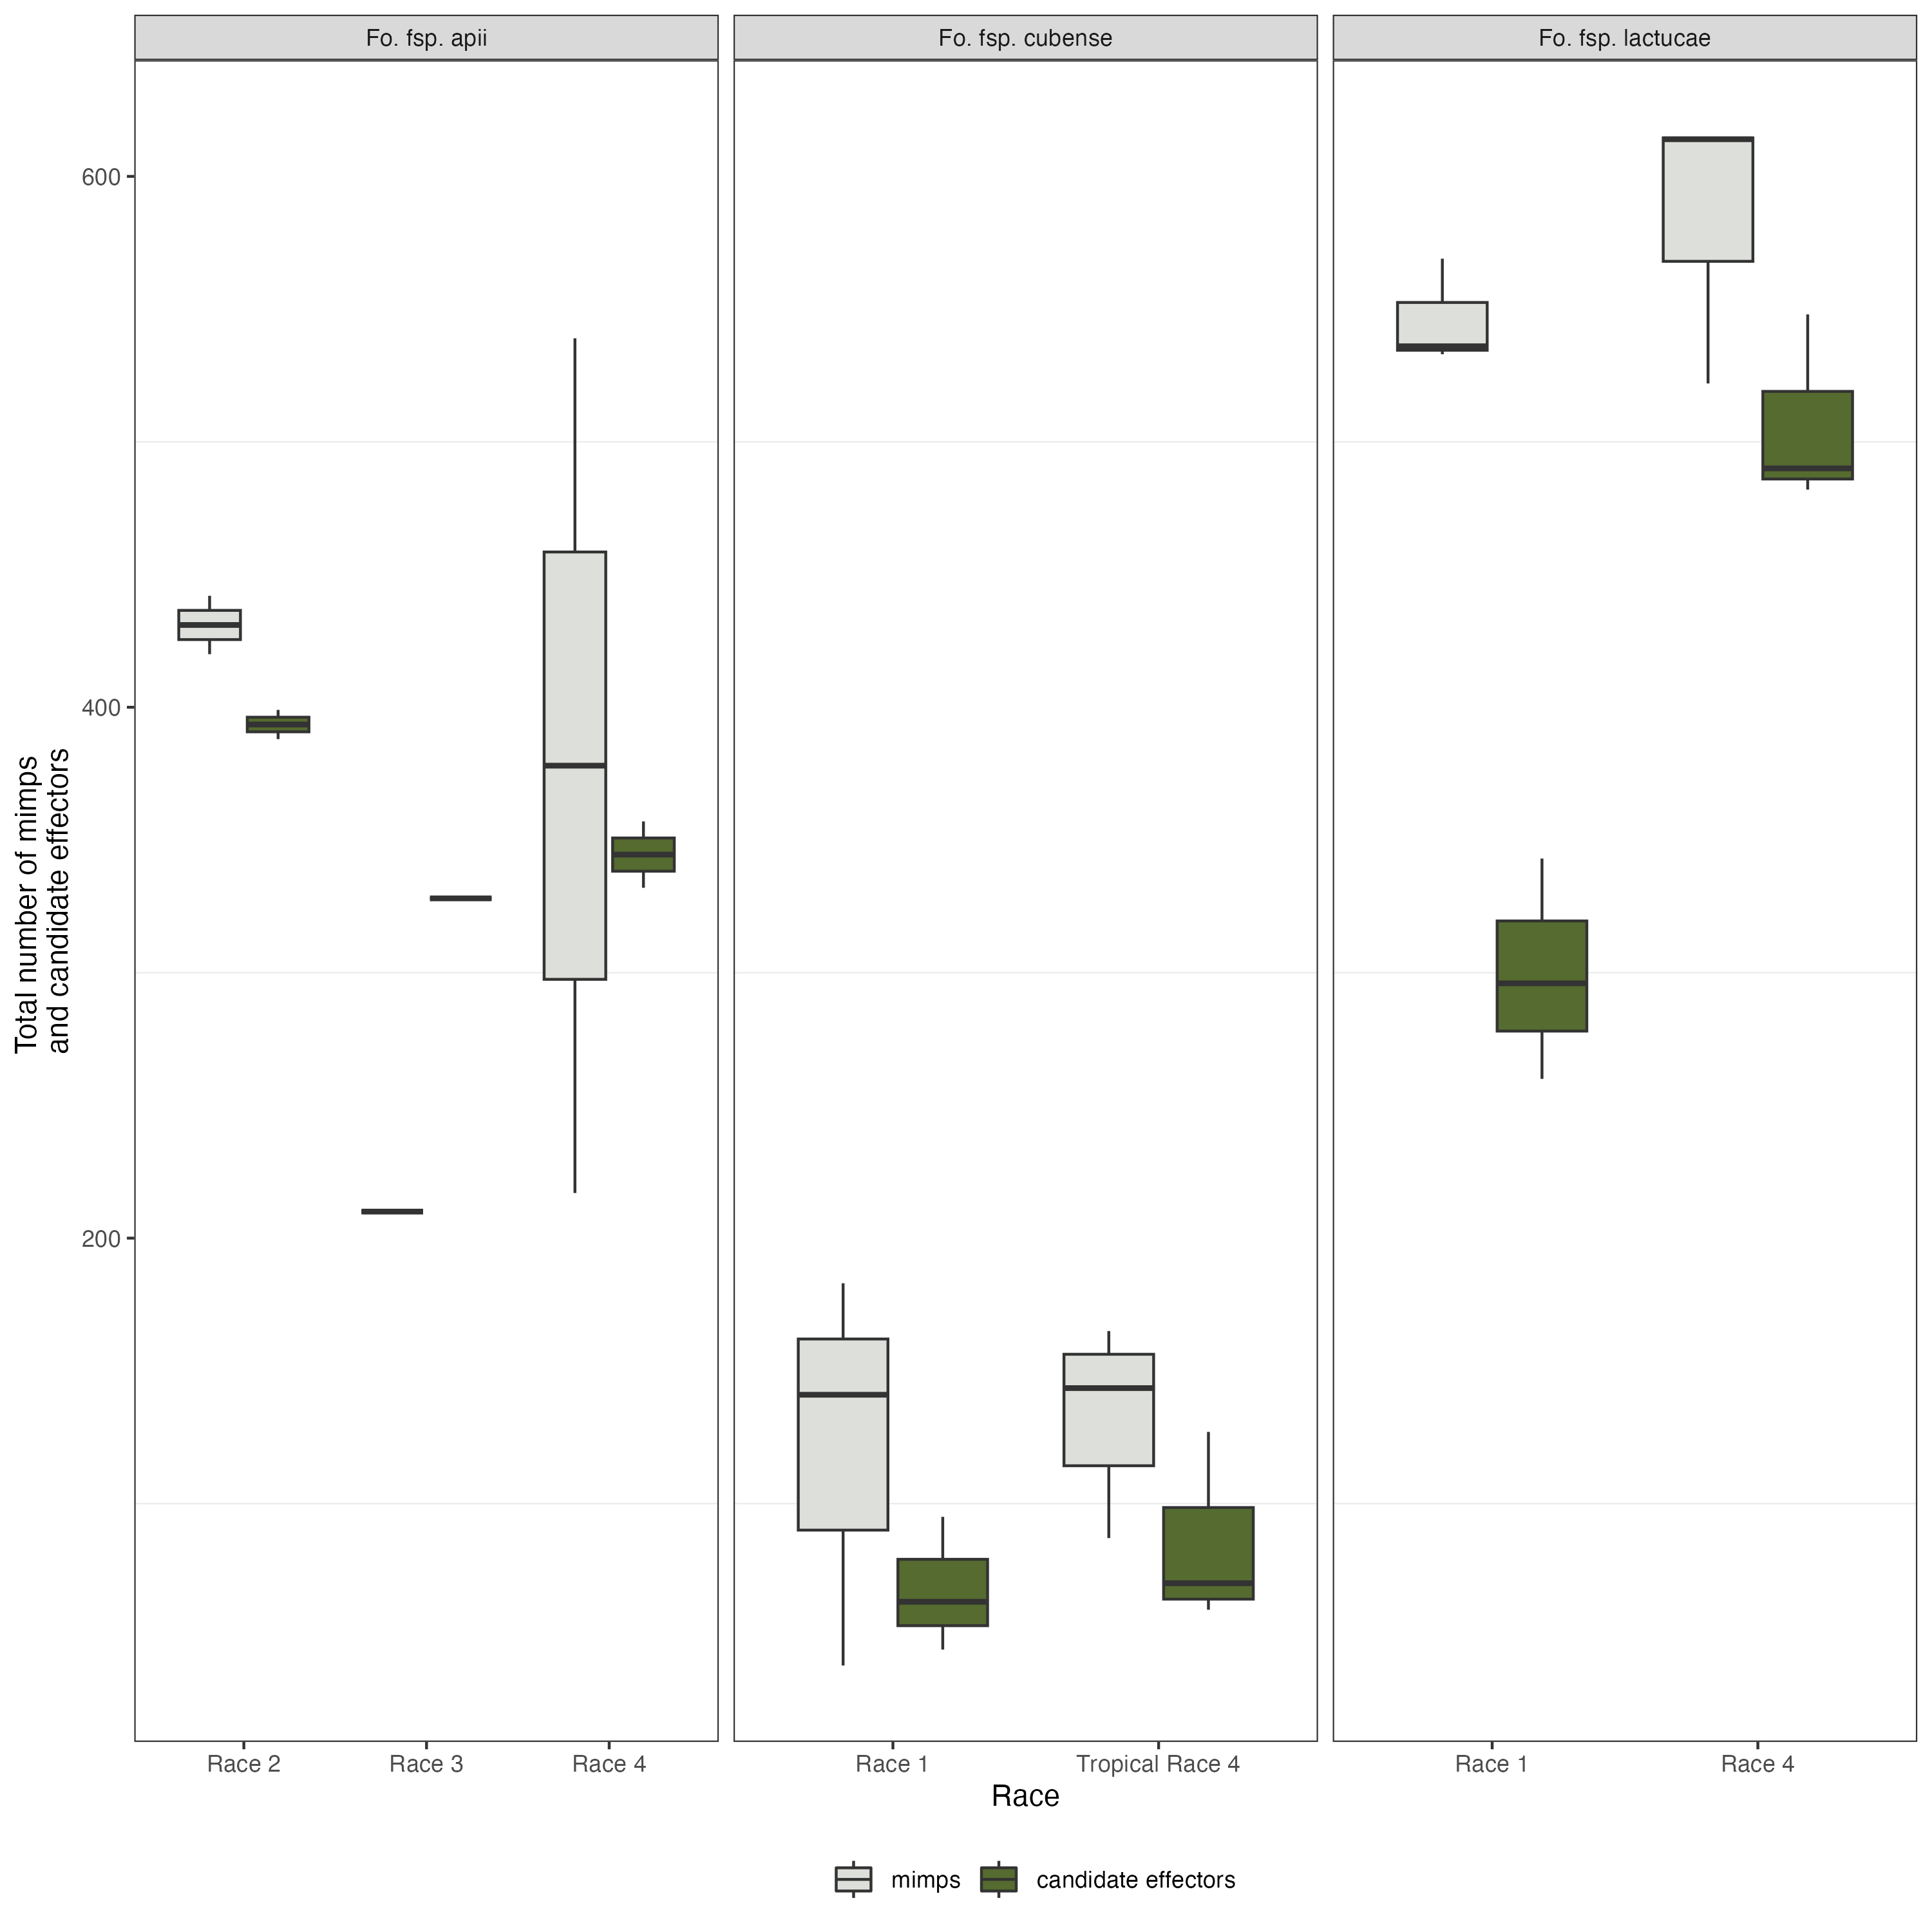
\includegraphics[width=\textwidth]{Figures/MimpsAndCandEffs_FspOfInterest.png}
    \caption[Boxplot of \ac{ce} and \ac{mimp} content in difference races of \ac{Foa}, \ac{Focub}, and \ac{Fola}.]{\textbf{\Acf{mimp} and \acf{ce} content in differs between races of \ac{Foa}, \ac{Focub}, and \ac{Fola}.} Black lines denote race median, whiskers indicate minimum and maximum, while boxes the first and third quartile. Only one genome assembly was included for \ac{Foa} \ac{r3}. The total number of genome assemblies per race was not equal; \ac{Foa} \ac{r2} = 2, \ac{r3} = 1, \ac{r4} = 2; \ac{Fola} \ac{r1} = 3, \ac{r4} = 3.}
    \label{fig:MaeiBoxPlot}
\end{figure}
\bigskip

\subsubsection{Distribution of \aclp{ce} from \ac{tnau} genome assemblies in \textit{Fusarium} pathogenic towards banana \ac{ce} sets}

To identify potentially orthologous \acp{ce} from \ac{tnau} genome assemblies in \textit{Fusarium} pathogenic towards banana, \ac{ce} sets from \ac{tnau} genome assemblies were searched for reciprocal best hits using MMseqs2 easy-rbh (v13.45111) against \ac{ce} identified through the \ac{maei} pipeline in some \textit{Fusarium} pathogenic towards banana  (\ac{Focub} isolates UK0001, 160527, VPRI44083, VPRI44084 and \ac{Fs} isolate FS66). Of the 333 \acp{ce} identified in \ac{tnau} S6 genome assembly, one was found in all \textit{Fusarium} pathogenic towards banana \ac{ce} sets searched, CE\_g74. Six \acp{ce} were found in all \ac{Focub} \ac{ce} sets searched, but not the \ac{Fs} FS66 set, one was identified in only the \ac{Fs} FS66 set. A further five four \acp{ce} from S6 were found in only one of the \ac{Focub} genome assembly \ac{ce} sets (Figure: \ref{fig:RBHupsets}a). 

Fewer of the \acp{ce} identified in \ac{tnau} genome assemblies for isolates S16 (n=289), S32 (n=314), and SY-2 (n=289) had reciprocal best hits \textcolor{red}{(WITHIN WHAT THRESHOLD???)} found in the \textit{Fusarium} pathogenic towards banana \ac{ce} sets.

\begin{figure}[ht!]
    \centering
    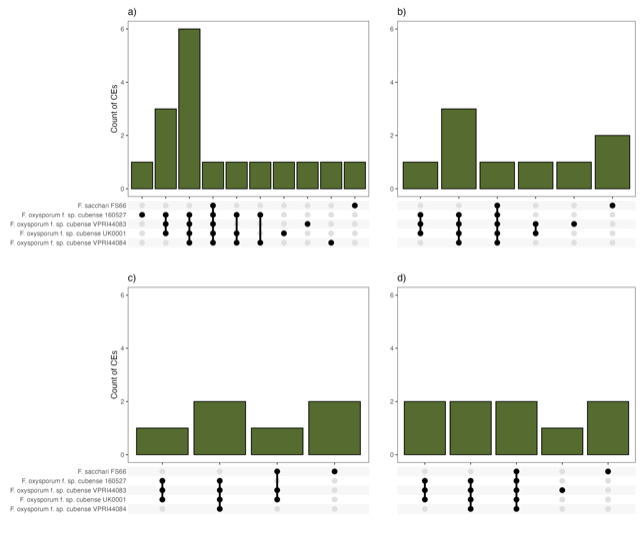
\includegraphics[width=\textwidth]{Figures/UpSetPlots.png}
    \caption[UpSet plot of reciprocal best hits of \ac{tnau} \acp{ce}  in \ac{Focub}, and \ac{Fs}.]{\textbf{UpSet plot of reciprocal best hits of \ac{tnau} \acp{ce}  in \ac{Focub}, and \ac{Fs}.}}
    \label{fig:RBHupsets}
\end{figure}

\subsection{\textit{Fusarium} from the same \textit{formae speciales} have a similar \acl{cec} profiles}

We identified 325 \acfp{cec} by grouping \ac{ce} identified using the \ac{maei} pipeline with $\geq65\% $ identity. On average, \acp{cec} contained 27 \acp{ce}, though the total number of sequences in a \ac{cec} ranged from 895 (n=1, CEC\_234) to one (n=80). A binary presence/absence matrix revealed that the total number of \ac{cec} varied among isolates (Table \ref{tab:CandEffNo}). The six \acp{ce} identified in the \ac{Fg} PH-1 genome assembly were distributed across six \acp{cec}, whereas the 603 \acp{ce} identified in the \ac{Foci} AJ615 genome assembly were distributed among 106 \acp{cec}. CEC\_80 emerged as a 'core \ac{cec}' for \textit{Fusarium}, as it was conserved across all \textit{Fusarium} genome assemblies, while eight core \acp{cec} were found among the \ac{Fo} genome assemblies. \ac{Focub} had an average of 45 \acp{cec} per genome assembly (range: 34 to 56), 16 of which were designated core \acp{cec}. The number of core \acp{cec} identified in \ac{Foci} genome assemblies was greater than that of \ac{Focub} at 64, though only two \ac{Foci} genome assemblies were included (isolate AJ615, CEC=106; isolate 3-2, CEC=99). The \ac{Foa} and \ac{Fola} genome assemblies have a similar number of core \acp{cec} at 54 and 56, respectively. Moreover, the average number of \acp{cec} in \ac{Foa} and \ac{Fola} was similar at  94 (range: 87 to 103) and 83 (range: 77 to 91), respectively.

Hierarchical clustering based on the \ac{cec} presence/absence matrix revealed that \ac{Fo} isolates tended to group within their respective \ac{fsp} (Figure \ref{fig:MaeiHeatmap}). However, notable exceptions are observed among \ac{Foa} and \ac{Foci}. \ac{Foa} \ac{r2} clusters separately from \ac{Foc} \ac{r3} and \ac{r4}. Similarly, the \ac{Foci} isolates group separately based on their \ac{cec} profile. This pattern mirrors the (\ac{tef}) phylogenetic analysis, where \ac{Foa} \ac{r2} does not sit within the same \ac{FOSC} clade as the \ac{Foa} \ac{r3} and \ac{r4} isolates  (Figure \ref{fig:TEF1aPhyloaMaei}). Likewise, the \ac{Foci} isolate 3-2 sits alongside \ac{Foa} \ac{r3} and \ac{r4} isolates in the \ac{tef} phylogeny, but \ac{Foci} isolate AJ615, sits in the same subclade as \textit{Fo. fsp. niveum}. 

\begin{sidewaysfigure}[hp!]
    \centering
    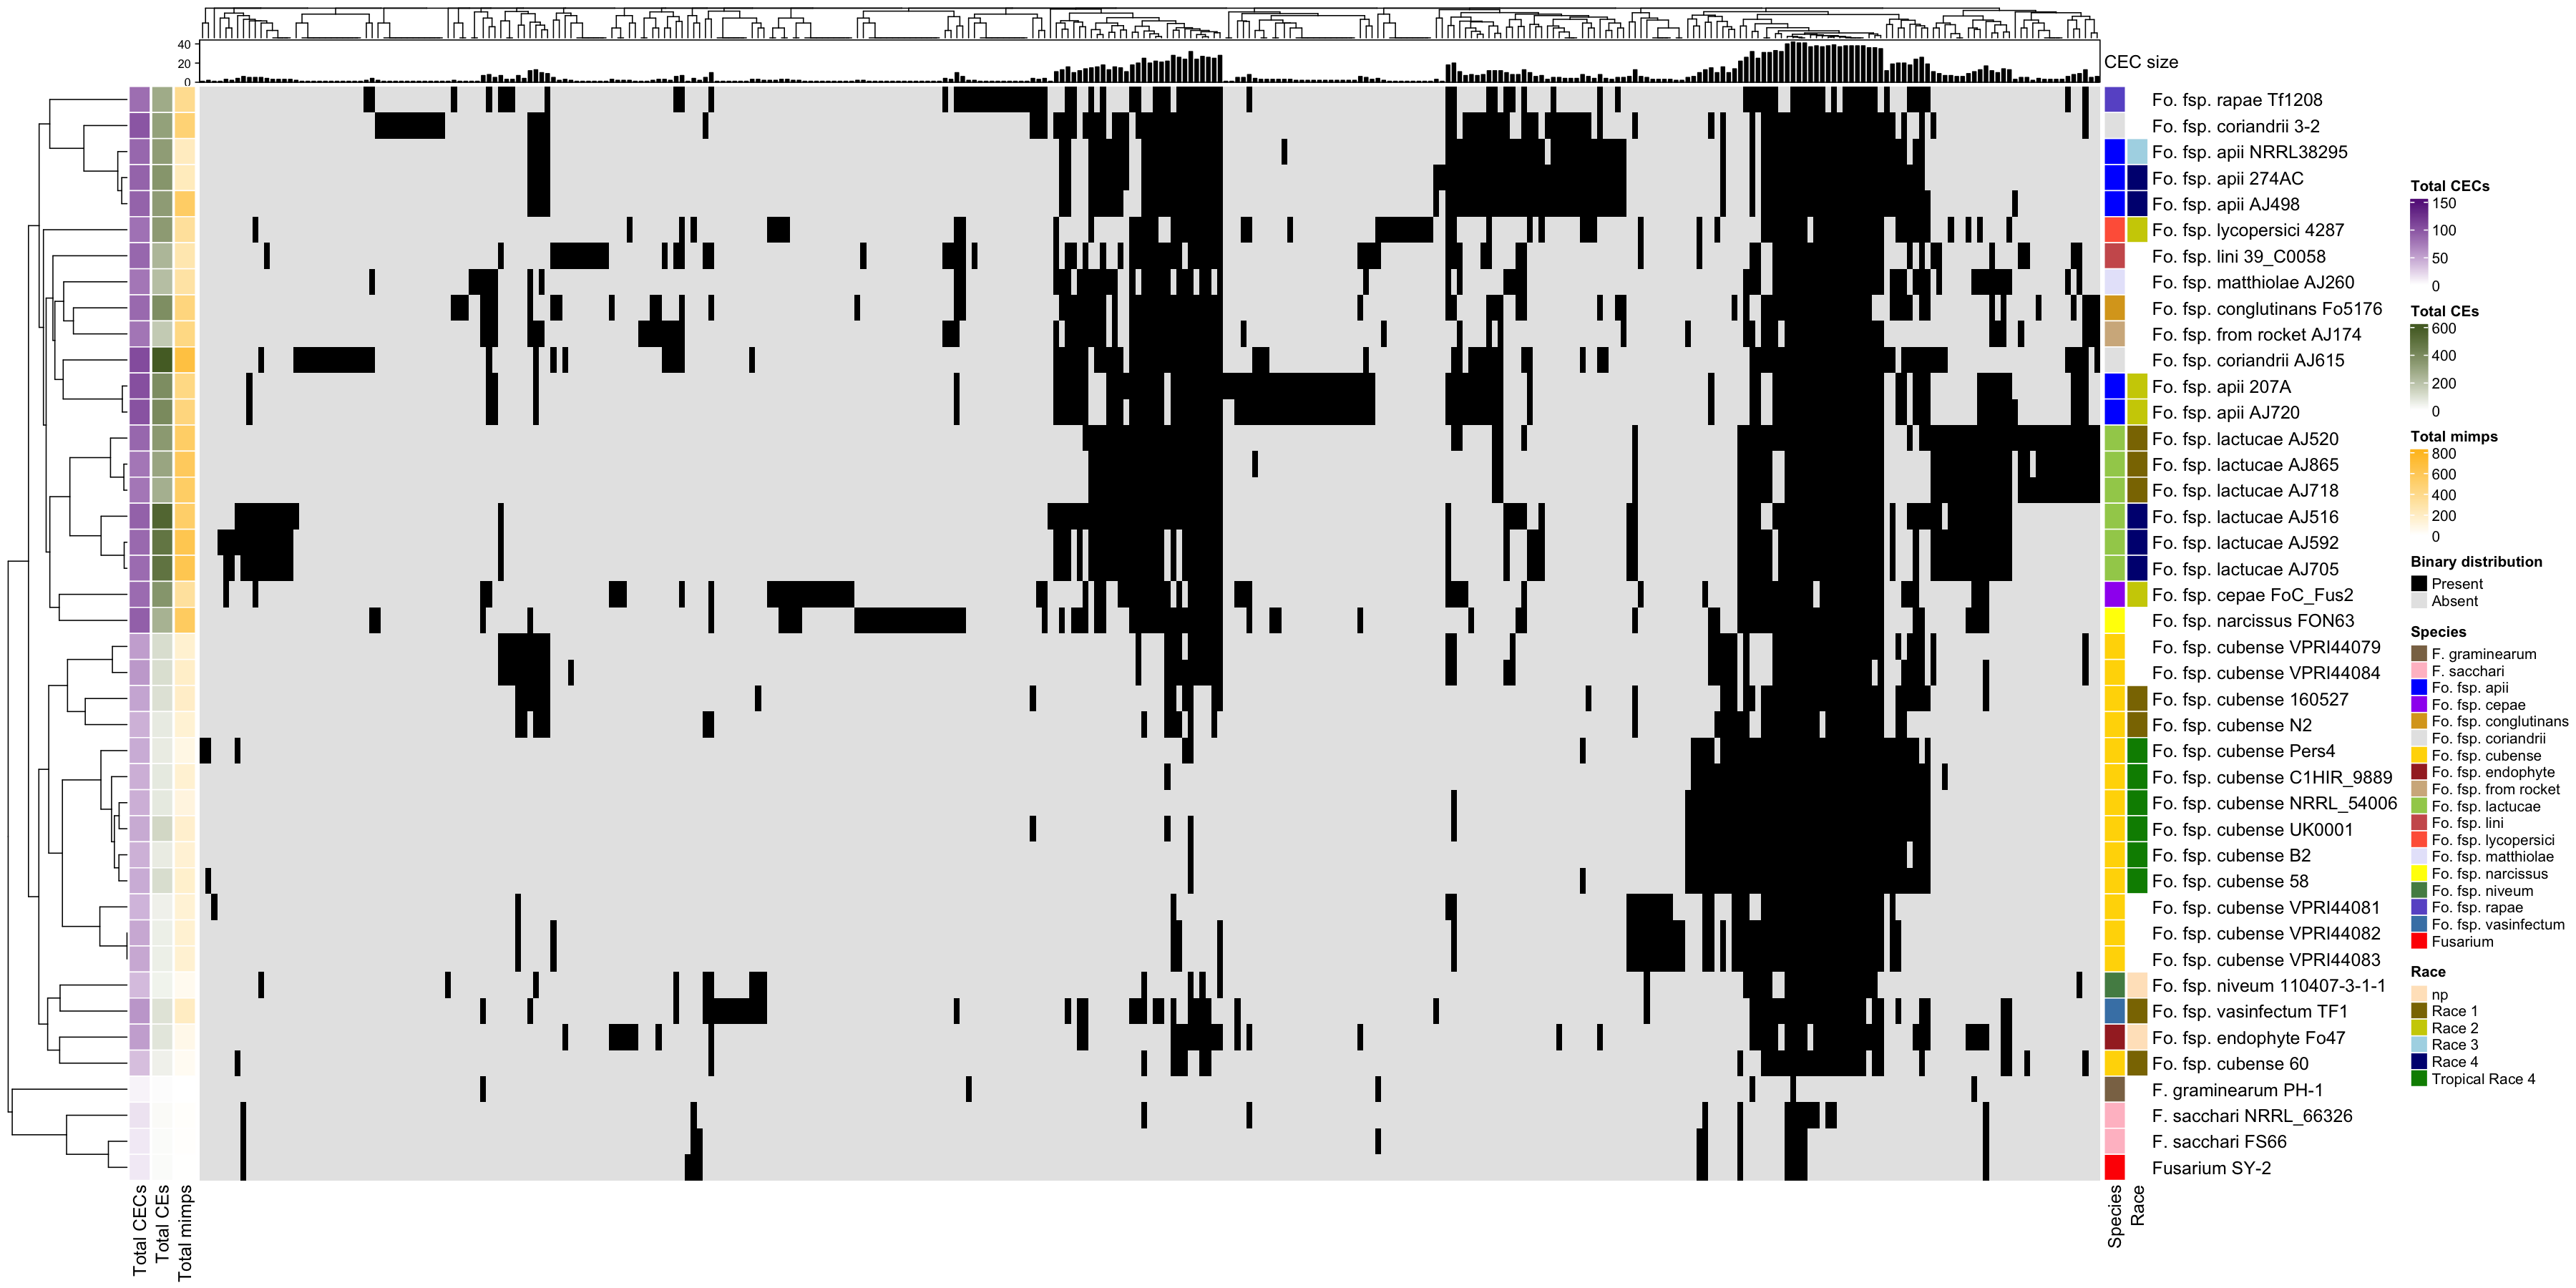
\includegraphics[width=\textwidth]{Figures/EffectorsHeatmap.png}
    \captionsetup{width=24cm}
    \caption[Heatmap of \acl{cec}s distribution in \textit{Fusarium} species.]{\textbf{Heatmap of \acf{cec} distribution in \textit{Fusarium} species.} \Acp{cec} were determined using CD-HIT (v4.8.1) at 80\% identity, following \ac{ce} identification using TBLASTN, (cut-off 1e-6 65\% identity and coverage threshold) and filtering using SignalP (v5.0b) and EffectorP (v2.1.0). np indicates non-pathogen.}
    \label{fig:MaeiHeatmap}
\end{sidewaysfigure}

\begin{figure}[hp!]
    \centering
    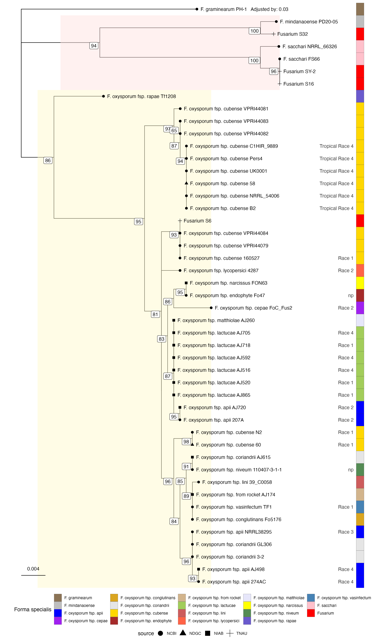
\includegraphics[width=12cm]{Figures/BasicTEFPhylo.png}
    \captionsetup{width=\textwidth}
    \caption[Maximum likelihood phylogeny from alignment of \Acl{tef} sequences from \textit{Fusarium} isolates included in candidate effector analysis.]{\textbf{Maximum likelihood phylogeny from alignment of \Acf{tef} sequences from \textit{Fusarium} isolates included in candidate effector analysis.} The tree is rooted through \textit{Fusarium graminearum} PH-1 \ac{tef}, which has had the branch length adjusted by 0.03. Branch lengths show expected number of substitutions per site. White boxes indicate bootstrap values from 1000 bootstrap replicates. \acl{Fs} clade is shown in light pink, the \ac{Fo} clade is shown in yellow. IQ-TREE2 (v2.2.0.3) determined best model of substitution  was TNe+G4. np indicates non-pathogen.}
    \label{fig:TEF1aPhyloaMaei}
\end{figure}

Though \ac{Foa} contained a set of 54 core \acp{cec} and \ac{Foci} had 64 core \acp{cec}; closely related \ac{Foa} and \ac{Foci} isolates shared more \ac{cec} and exhibited comparable \ac{cec} profiles. Specifically, \ac{Foci} 3-2, along with \ac{Foa} \ac{r3} and \ac{r4} isolate genome assemblies formed a monophyletic group (Appendix \ref{fig:Maei_celeryandcoriander}). The \ac{cec} profile of \ac{Foa} \ac{r3} and \ac{r4} genome assemblies was nearly identical, and was similar to that of \ac{Foci} 3-2 (Figure \ref{fig:MaeiHeatmap}). A combined total of 93 \acp{cec} were identified in \ac{Foa} \ac{r3} and \ac{r4}, with 85 being common to all \ac{Foa} \ac{r3} and \ac{r4} isolates. Of the eight remaining \acp{cec}, four were identified in only one of \ac{Foa} \ac{r4} assemblies, while four were exclusive to \ac{Foa} \ac{r3}. \ac{Foci} 3-2 shared a total of 73 \acp{cec} with \ac{Foa} \ac{r3} and \ac{r4}, nine more \acp{cec} than it shared with the other \ac{Foci} isolate, AJ615. 


\subsection{\Acl{ce} compliment of \textit{Fusarium} isolates pathogenic towards banana.} 

 Three \acp{mimp} and 12 \acp{ce} were identified in the genome assembly for the \ac{tnau} isolate, SY-2. The \ac{cec} profile of SY-2 was similar to that of the \ac{Fs} genome assemblies for isolates FS66 and NRRL\_66326, with nine core \acp{cec} identified in SY-2, FS66, and NRRL\_66326.  Interestingly, the number of \acp{cec} in each the \ac{Fs} (FS66 = 12 and NRRL\_66326 = 15) and SY-2 genome assembly was consistently less than the number of \acp{cec} identified in the non-pathogenic \ac{Fo} genome assemblies (Fo47 = 53 and 110407-3-1-1 = 36) (Figure \ref{fig:CECcount}). Four \acp{cec} were conserved across all genome assemblies from isolates pathogenic towards banana (the \ac{Fs}, \ac{Focub}, and SY-2 genome assemblies). Further, the SY-2 and \ac{Fs} genome assemblies clustered in to a separate \ac{cec} profile group from the genome assemblies in the \ac{FOSC}, which mirrors the \ac{tef} phylogeny, where SY-2 and \ac{Fs} genome assemblies sit in a separate clade from the genomes in the \ac{FOSC}.

The number of \acp{cec} identified in the \ac{Focub} genome assemblies was comparable to the non-pathogenic \ac{Fo} genome assemblies, and \ac{Focub} genome assemblies clustered alongside the non-pathogenic \ac{Fo} genome assemblies based on \ac{cec} profile (Figure \ref{fig:MaeiHeatmap}). A similar number of \acp{cec} were identified in all of the \ac{Focub4} genome assemblies ranging from 42 (B2) to 46 (UK0001). The number of \acp{cec} in the \ac{Focub1} genome assemblies varied a little more, with 34 identified in isolate 60, and 49 identified in isolate 160527 (Figure \ref{fig:CECcount}). 

\begin{figure}[ht!]
    \centering
    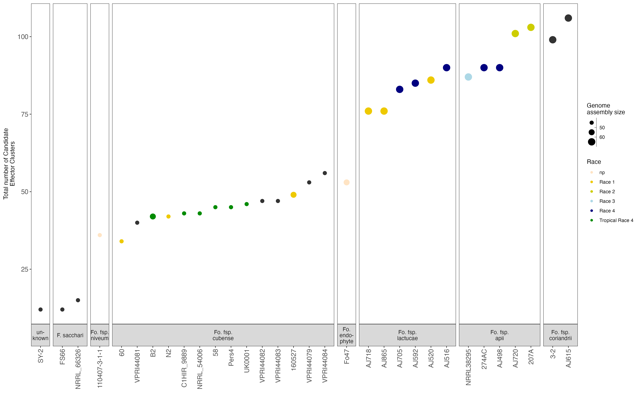
\includegraphics[width=\textwidth]{Figures/CecDistribinFspOfInterest.png}
    \captionsetup{width=\textwidth}
    \caption[\Acl{cec} count across \acl{Fs}, \ac{tnau} isolate SY-2, \acl{Fo} non-pathogens, and the \ac{Fo} \acp{fsp} \textit{apii, coriandrii, cubense} and \textit{lactucae}..]{\textbf{\Acf{cec} count across \acl{Fs}, \ac{tnau} isolate SY-2, \acf{Fo} non-pathogens, and the \ac{Fo} \acp{fsp} \textit{apii, coriandrii, cubense} and \textit{lactucae}.} Point size indicates genome assembly size and colour indicates race. Genome assemblies for which race has not been assigned are shown in black. np indicates non-pathogen}
    \label{fig:CECcount}
\end{figure}

Though \ac{Focub} assemblies generally clustered together based on their \ac{cec} profiles, variations between races and isolates were observed. \ac{Focub} 60, was the only \ac{Focub} assembly to cluster separately from the other \ac{Focub} assemblies based on \ac{cec} profile. \ac{Focub} 60 is reported to be a \ac{r1} isolate \parencite{Yun2019}, but the \ac{cec} profile of \ac{Focub} 60 is more similar to the \ac{Fo} endophyte, Fo47. The remaining \ac{Focub} genome assemblies sit within one \ac{Focub} \ac{CEC} profile group (Figure \ref{fig:MaeiHeatmap}), which divides into three further \ac{Focub} \ac{cec} profile groups. The first \ac{Focub} \ac{cec} profile group contains two \ac{Focub1} genome assemblies (N2 and 160527) as well as VPR144079 and VPR144084. Phylogenetic analysis based on the \ac{tef} gene revealed a polyphyletic evolutionary history for \ac{Focub}, which has also been observed by \textcite{Maryani2019, Mostert2022}. Based on the \ac{tef} phylogeny, 160527, VPR144079, and VPR144084 form a monophyletic clade (along \ac{tnau} isolate, S6). The \ac{Focub1} isolates N2 and 60, sit in a separate clade and are more closely related to other \ac{Fo} \acp{fsp} than the \ac{Focub1} isolates 160527, VPR144079, and VPR144084. However, the \ac{cec} profile does not reflect the \ac{tef} phylogeny (Figure \ref{fig:MaeiHeatmap-banana}). VPR144079 and VPR144084 have very similar \ac{cec} profiles, but 160527 \ac{cec} profile resembles that of N2 more than that of VPR144079 and VPR144084. 

The second \ac{Focub} \ac{cec} profile cluster contains all \ac{Focub4} genome assemblies. A combined set of 52 \acp{cec} were identified in the \ac{Focub4} genome assemblies, with a core set of 38 \acp{cec}. The remaining  14 \acp{cec} were not identified in all \ac{Focub4} genome assemblies. The third  \ac{Focub} \ac{cec} profile cluster is comprised of  VPR144081, VPR144082, and VPR144083, 38 core \acp{cec} were identified from the 49 \acp{cec} among these isolates. Further, these isolates are from the same lineage as \ac{Focub4}, but display a slightly different \ac{cec} profile (Figure \ref{fig:MaeiHeatmap-banana}). VPR144081, VPR144082, and VPR144083 share 27 \acp{cec} with the \ac{Focub4} assemblies. 

\begin{sidewaysfigure}[htp!]
    \centering
    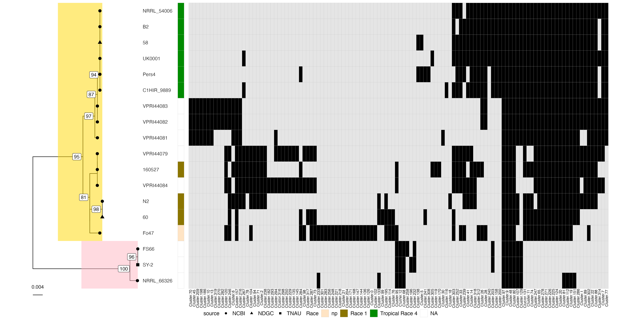
\includegraphics[width=\textwidth]{Figures/HeatmapAndPhylo_BananaPathOnly.png}
    \captionsetup{width=24cm}
    \caption[Maximum likelihood phylogeny from alignment of \Acl{tef} sequences from isolates  causing \acl{fwb} alongside respective \acl{cec} profiles.]{\textbf{Maximum likelihood phylogeny from alignment of \Acf{tef} sequences from isolates causing \acl{fwb} alongside respective \acf{cec} profiles.} \ac{FFSC} shown in pink, \ac{FOSC} shown in yellow. The \ac{Fo} non-pathogen, Fo47 was also included. Branch length show expected number of substitutions per site. White boxes indicate bootstrap values from 1000 bootstrap replicates. IQ-TREE2 (v2.2.0.3) best model of substitution; TNe+G4. \Acp{cec} were determined using CD-HIT (v4.8.1) at 80\% identity, following \ac{ce} identification using TBLASTN, (cut-off 1e-6 65\% identity and coverage threshold) and filtering using SignalP (v5.0b) and EffectorP (v2.1.0). np indicates non-pathogen.}
    \label{fig:MaeiHeatmap-banana}
\end{sidewaysfigure}


\textcolor{red}{Have a look at some of the interesting ones (race specific) and show BLAST/HMM/Interproscan results.}

% - Pred functions of race specific effectors?
\subsection{Variation in \acl{Fola} effector compliment.}

Although the \ac{Fo} genome assemblies typically clustered into \ac{cec} profile groups by \acp{fsp} then race, assemblies from the same race did not consistently have identical \ac{cec} profiles. The \ac{Fola} assemblies included in this study demonstrate this well. All \ac{Fola} isolates formed a monophyletic clade based on the \ac{tef} phylogeny with no obvious race grouping. The \ac{Fola} genome assemblies also clustered together based on \ac{cec} profile, separating into two race-specific clusters; the \ac{Fola} \ac{r4} \ac{cec} profile cluster, which had a mean \ac{cec} count of 86  (range: 83 to 90), and the \ac{Fola} \ac{r1} \ac{cec} profile cluster, which had a mean \ac{cec} count of 79 (range: 76 to 86). Between all the \ac{Fola} \ac{r4} isolates, there is a core set of 77 \acp{cec}. The \ac{Fola} \ac{r4} isolates AJ592 and AJ705 displayed very similar \ac{cec} profiles, sharing 84 \acp{cec}, with AJ592 containing an additional 2 \acp{cec} compared to AJ705 (CEC\_241 and CEC\_47). The \ac{cec} profile of AJ516 is less like AJ592 and AJ705, containing an additional 20 \ac{cec} not identified in AJ592 and AJ705 (Figure \ref{fig:MaeiHeatmap-lettuce}). Of the 88 \acp{cec} identified in \ac{Fola} \ac{r2}, 76 are core \acp{cec}. \ac{Fola} \ac{r1} AJ520 shows an expanded \ac{cec} profile compared to AJ865 and AJ718, with 87 \acp{cec} identified (AJ865 = 77 \acp{cec}, and AJ718 = 77 \acp{cec}).

\begin{sidewaysfigure}[htp!]
    \centering
    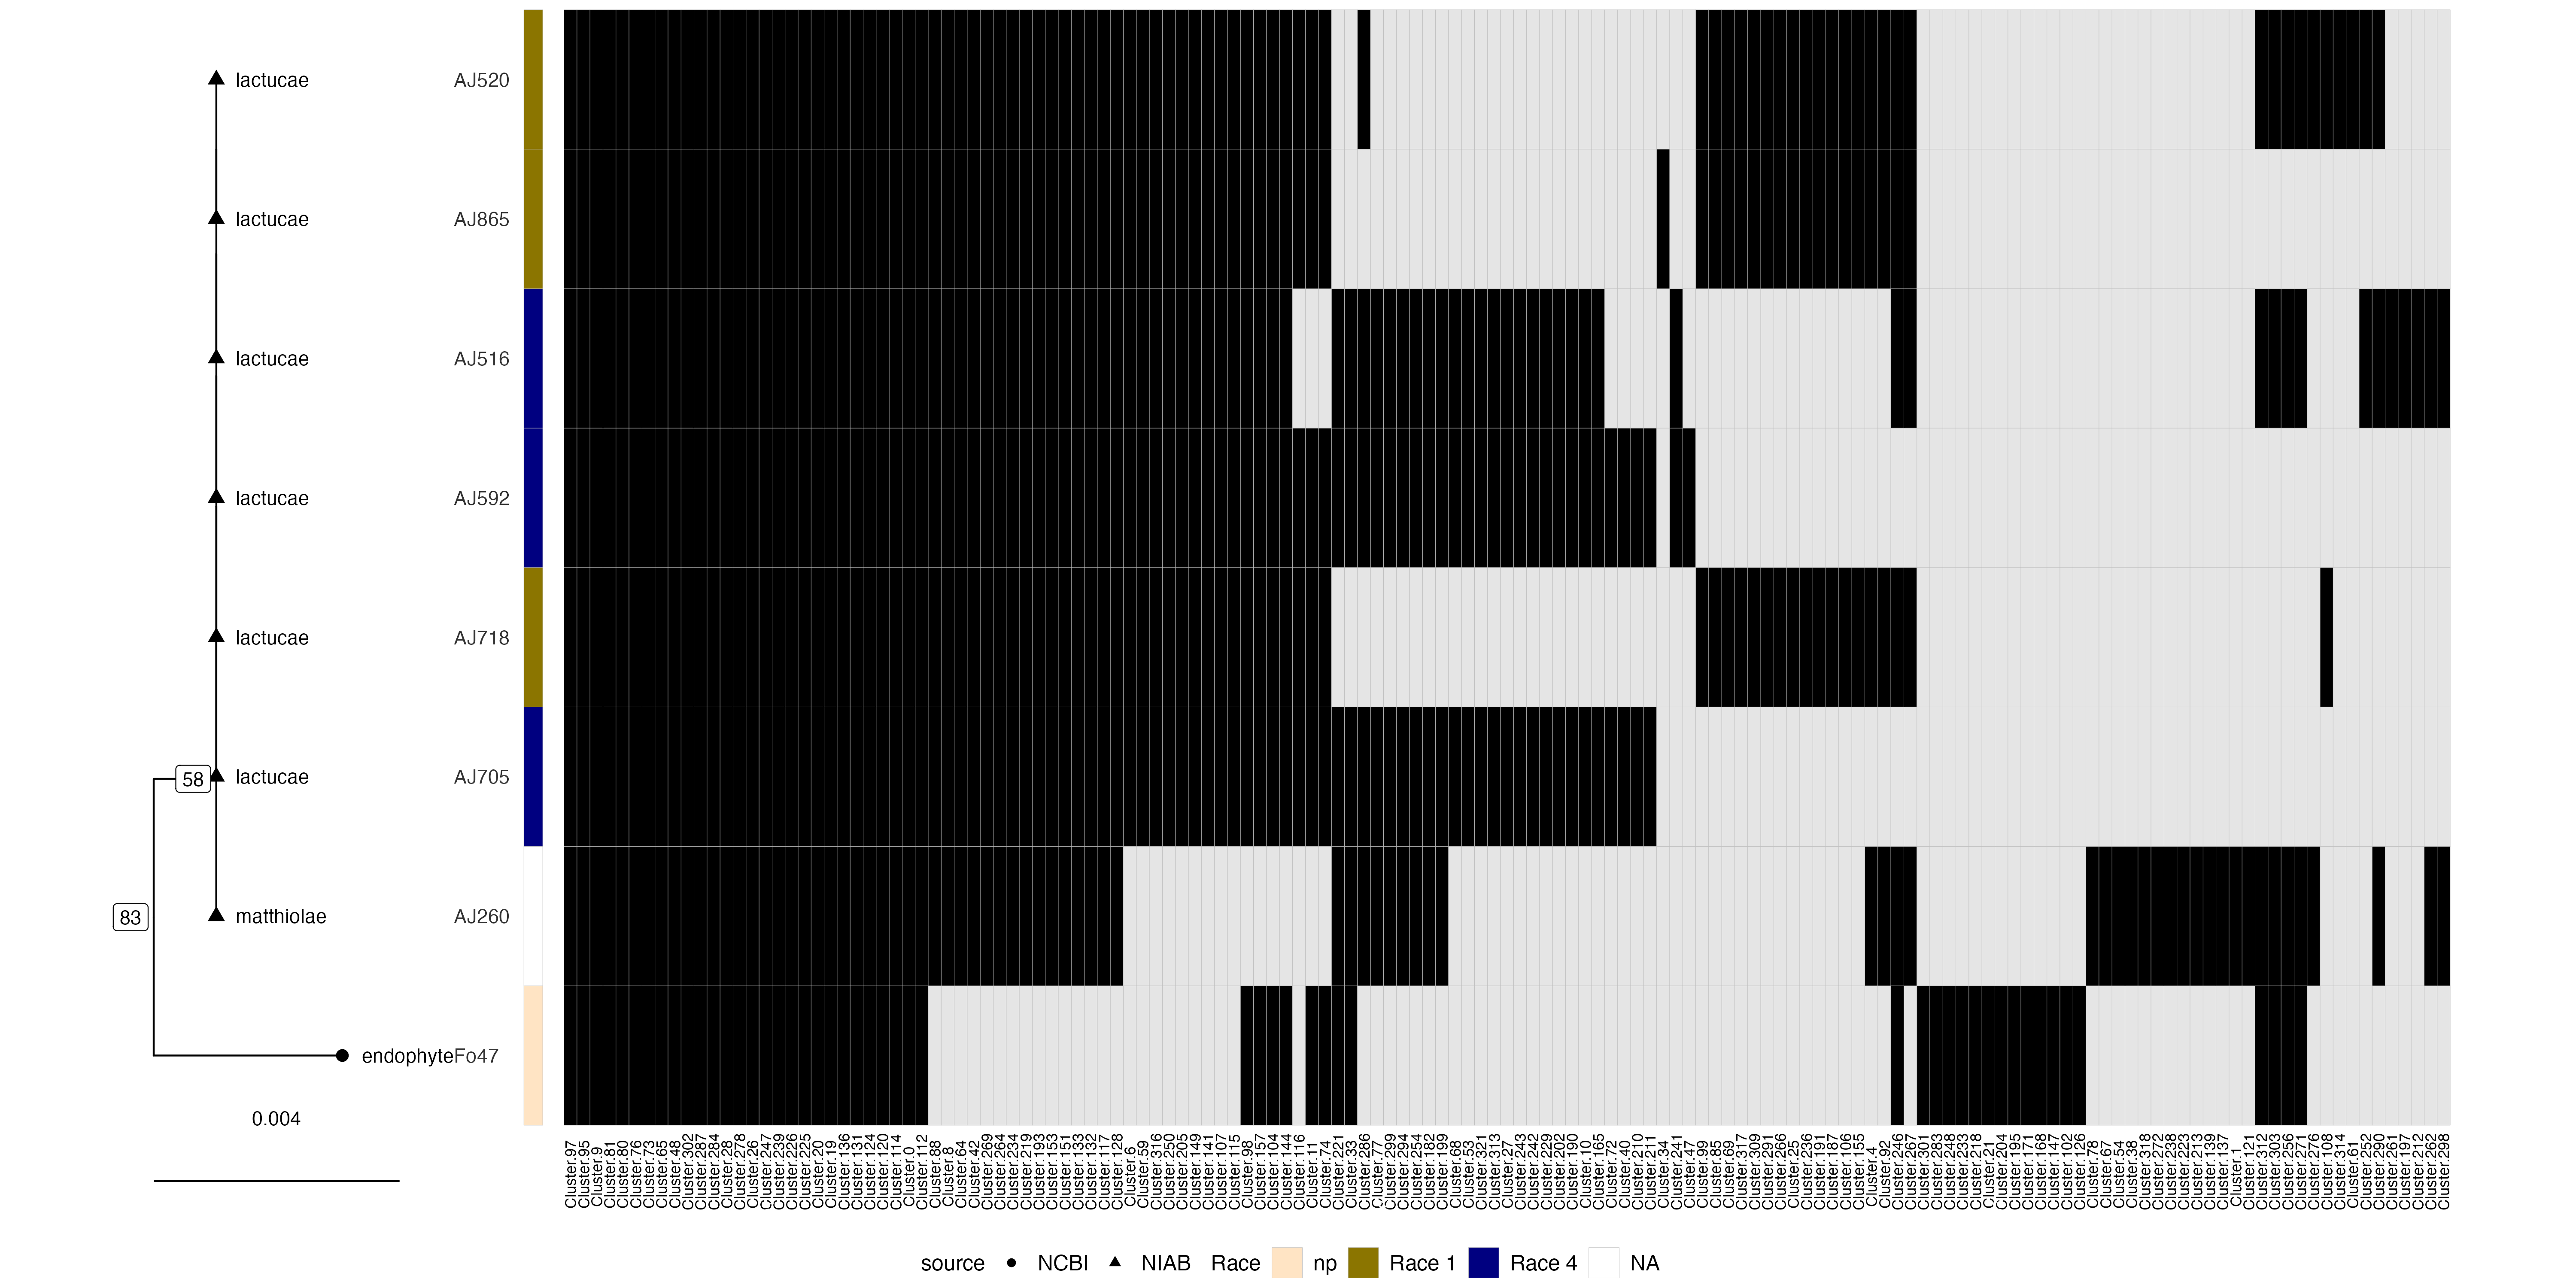
\includegraphics[width=\textwidth]{Figures/HeatmapAndPhylo_LactucaeOnly.png}
    \captionsetup{width=24cm}
    \caption[Maximum likelihood phylogeny from alignment of \Acl{tef} sequences from \acl{Fola} and \acl{Foci} isolates alongside respective \acl{cec} profiles.]{\textbf{Maximum likelihood phylogeny from alignment of \Acf{tef} sequences from \acf{Fola} isolates alongside respective \acf{cec} profiles.}  Branch length show expected number of substitutions per site. White boxes indicate bootstrap values from 1000 bootstrap replicates. IQ-TREE2 (v2.2.0.3) best model of substitution; TNe+G4. \Acp{cec} were determined using CD-HIT (v4.8.1) at 80\% identity, following \ac{ce} identification using TBLASTN, (cut-off 1e-6 65\% identity and coverage threshold) and filtering using SignalP (v5.0b) and EffectorP (v2.1.0). \ac{Fo} isolate Fo47 was included for \ac{cec} profile comparison against non-pathogen. np indicates non-pathogen.}
    \label{fig:MaeiHeatmap-lettuce}
\end{sidewaysfigure}

\subsubsection{Diverse \textit{SIX8} gene phylogenies reveal variability within \acl{Fola} \acl{r4} isolates.}

The differences observed in \ac{cec} profile among isolates from the same race, (e.g. \ac{Fola} \ac{r4} AJ516 vs AJ592 and AJ705), may be an artefact of genome assembly, but may also be due to differences in \ac{ce} complement of \ac{Fo} \ac{fsp} strains from the same race. This was explored in  \ac{Fola} races, where we observed sequence variation and differences in copy number of \textit{SIX8} (only found in \ac{Fola} \ac{r4}), \textit{SIX9}, and \textit{SIX14} homologues. In each \ac{Fola} \ac{r4} genome assembly, a single copy of \textit{SIX8} was identified. \textit{SIX8} in AJ592 and AJ705 were identical, but when aligned to \textit{SIX8} from AJ516, 16 base substitutions and one indel (position 528 to 535) were identified (Figure \ref{fig:lactucae-six8}). The two distinct variants of the \textit{SIX8} sequence in \ac{Fola} \ac{r4} were consistently detected among 39 isolates collected from Italy, Ireland, the Netherlands, Spain, and the UK. Among these isolates, 23 exhibited an identical sequence to the \ac{Fola} \ac{r4} isolate AJ516, while six isolates displayed the sequence shared by AJ592 and AJ705 (data not presented). The \textit{SIX8} sequences from \ac{Fola} were  most closely related to the \ac{Fo} isolate from rocket (AJ174), \ac{Fo} \ac{fsp} \textit{conglutinans} (Fo5176), and \ac{Fo} \ac{fsp} \textit{matthiolae} (AJ260).

\begin{figure}[htp!]
    \centering
    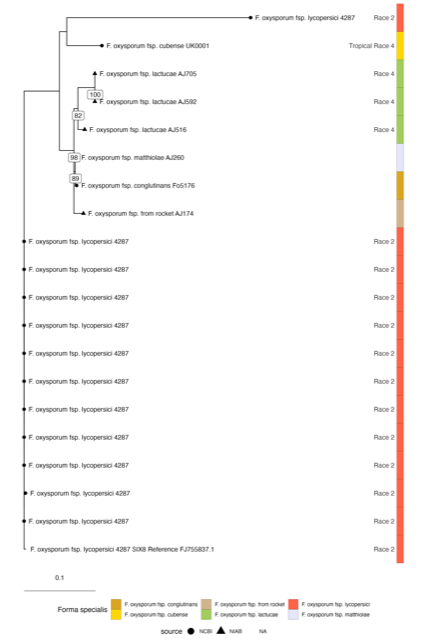
\includegraphics[width=13cm]{Figures/lactucaeSIX8tree.png}
    \captionsetup{width=\textwidth}
    \caption[Maximum likelihood phylogeny from alignment of \textit{SIX8} sequences from \acl{Fo} reveals differences in \acl{Fola} \acl{r4} \textit{SIX8}.]{\textbf{Maximum likelihood phylogeny from alignment of \textit{SIX8} sequences from \acf{Fo} reveals differences in \acf{Fola} \acf{r4} \textit{SIX8}.}  Branch length show expected number of substitutions per site. White boxes indicate bootstrap values from 1000 bootstrap replicates. IQ-TREE2 (v2.2.0.3) best model of substitution; K2P+G4. The tree is rooted with the reference sequence FJ755837.1 from \ac{Foly} \textit{SIX8}.}
    \label{fig:lactucae-six8}
\end{figure}

\textit{SIX9} copy number varied between \ac{Fola} races and isolates, with two copies identified in \ac{r1}, four copies identified in \ac{r4} AJ516, and five copies identified in \ac{r4} isolates AJ592 and AJ705. Though there was variation between the two copies of \textit{SIX9} in the \ac{Fola} \ac{r1} isolates, which were in separate clades, there was no variation in these copies between isolates (Group 1 and Group 3, Figure \ref{fig:lactucae-six9}). One of the \textit{SIX9} copies appears to have been duplicated in \ac{Fola} \ac{r4}, with two copies of \textit{SIX9} in each isolate that are identical to the \ac{Fola} \ac{r1} copy (Group 3, Figure \ref{fig:lactucae-six9}). Additional copies of \textit{SIX9}, found in all the \ac{Fola} \ac{r4} isolates (but absent in \ac{Fola} \ac{r1}), exhibited similarity to \textit{SIX9} copies identified in \ac{Fo} from rocket (AJ174), \ac{Fo} \acp{fsp} \textit{coriandrii} (3-2), \textit{conglutinans} (Fo5176), and \textit{matthiolae} (AJ260), mirroring the pattern observed with \textit{SIX8} (Group 2, Figure \ref{fig:lactucae-six9}). Additionally, copies of \textit{SIX9} identified in \ac{Fola} \ac{r4} exhibited similarity to a copy of \textit{SIX9} in \ac{Foci} (Group 4, Figure \ref{fig:lactucae-six9}). A further \textit{SIX9} sequence variant was identified in \ac{Fola} \ac{r4} isolates AJ592 and AJ705, but not AJ516 (Group 1, Figure \ref{fig:lactucae-six9}). 

\begin{figure}[htp!]
    \centering
    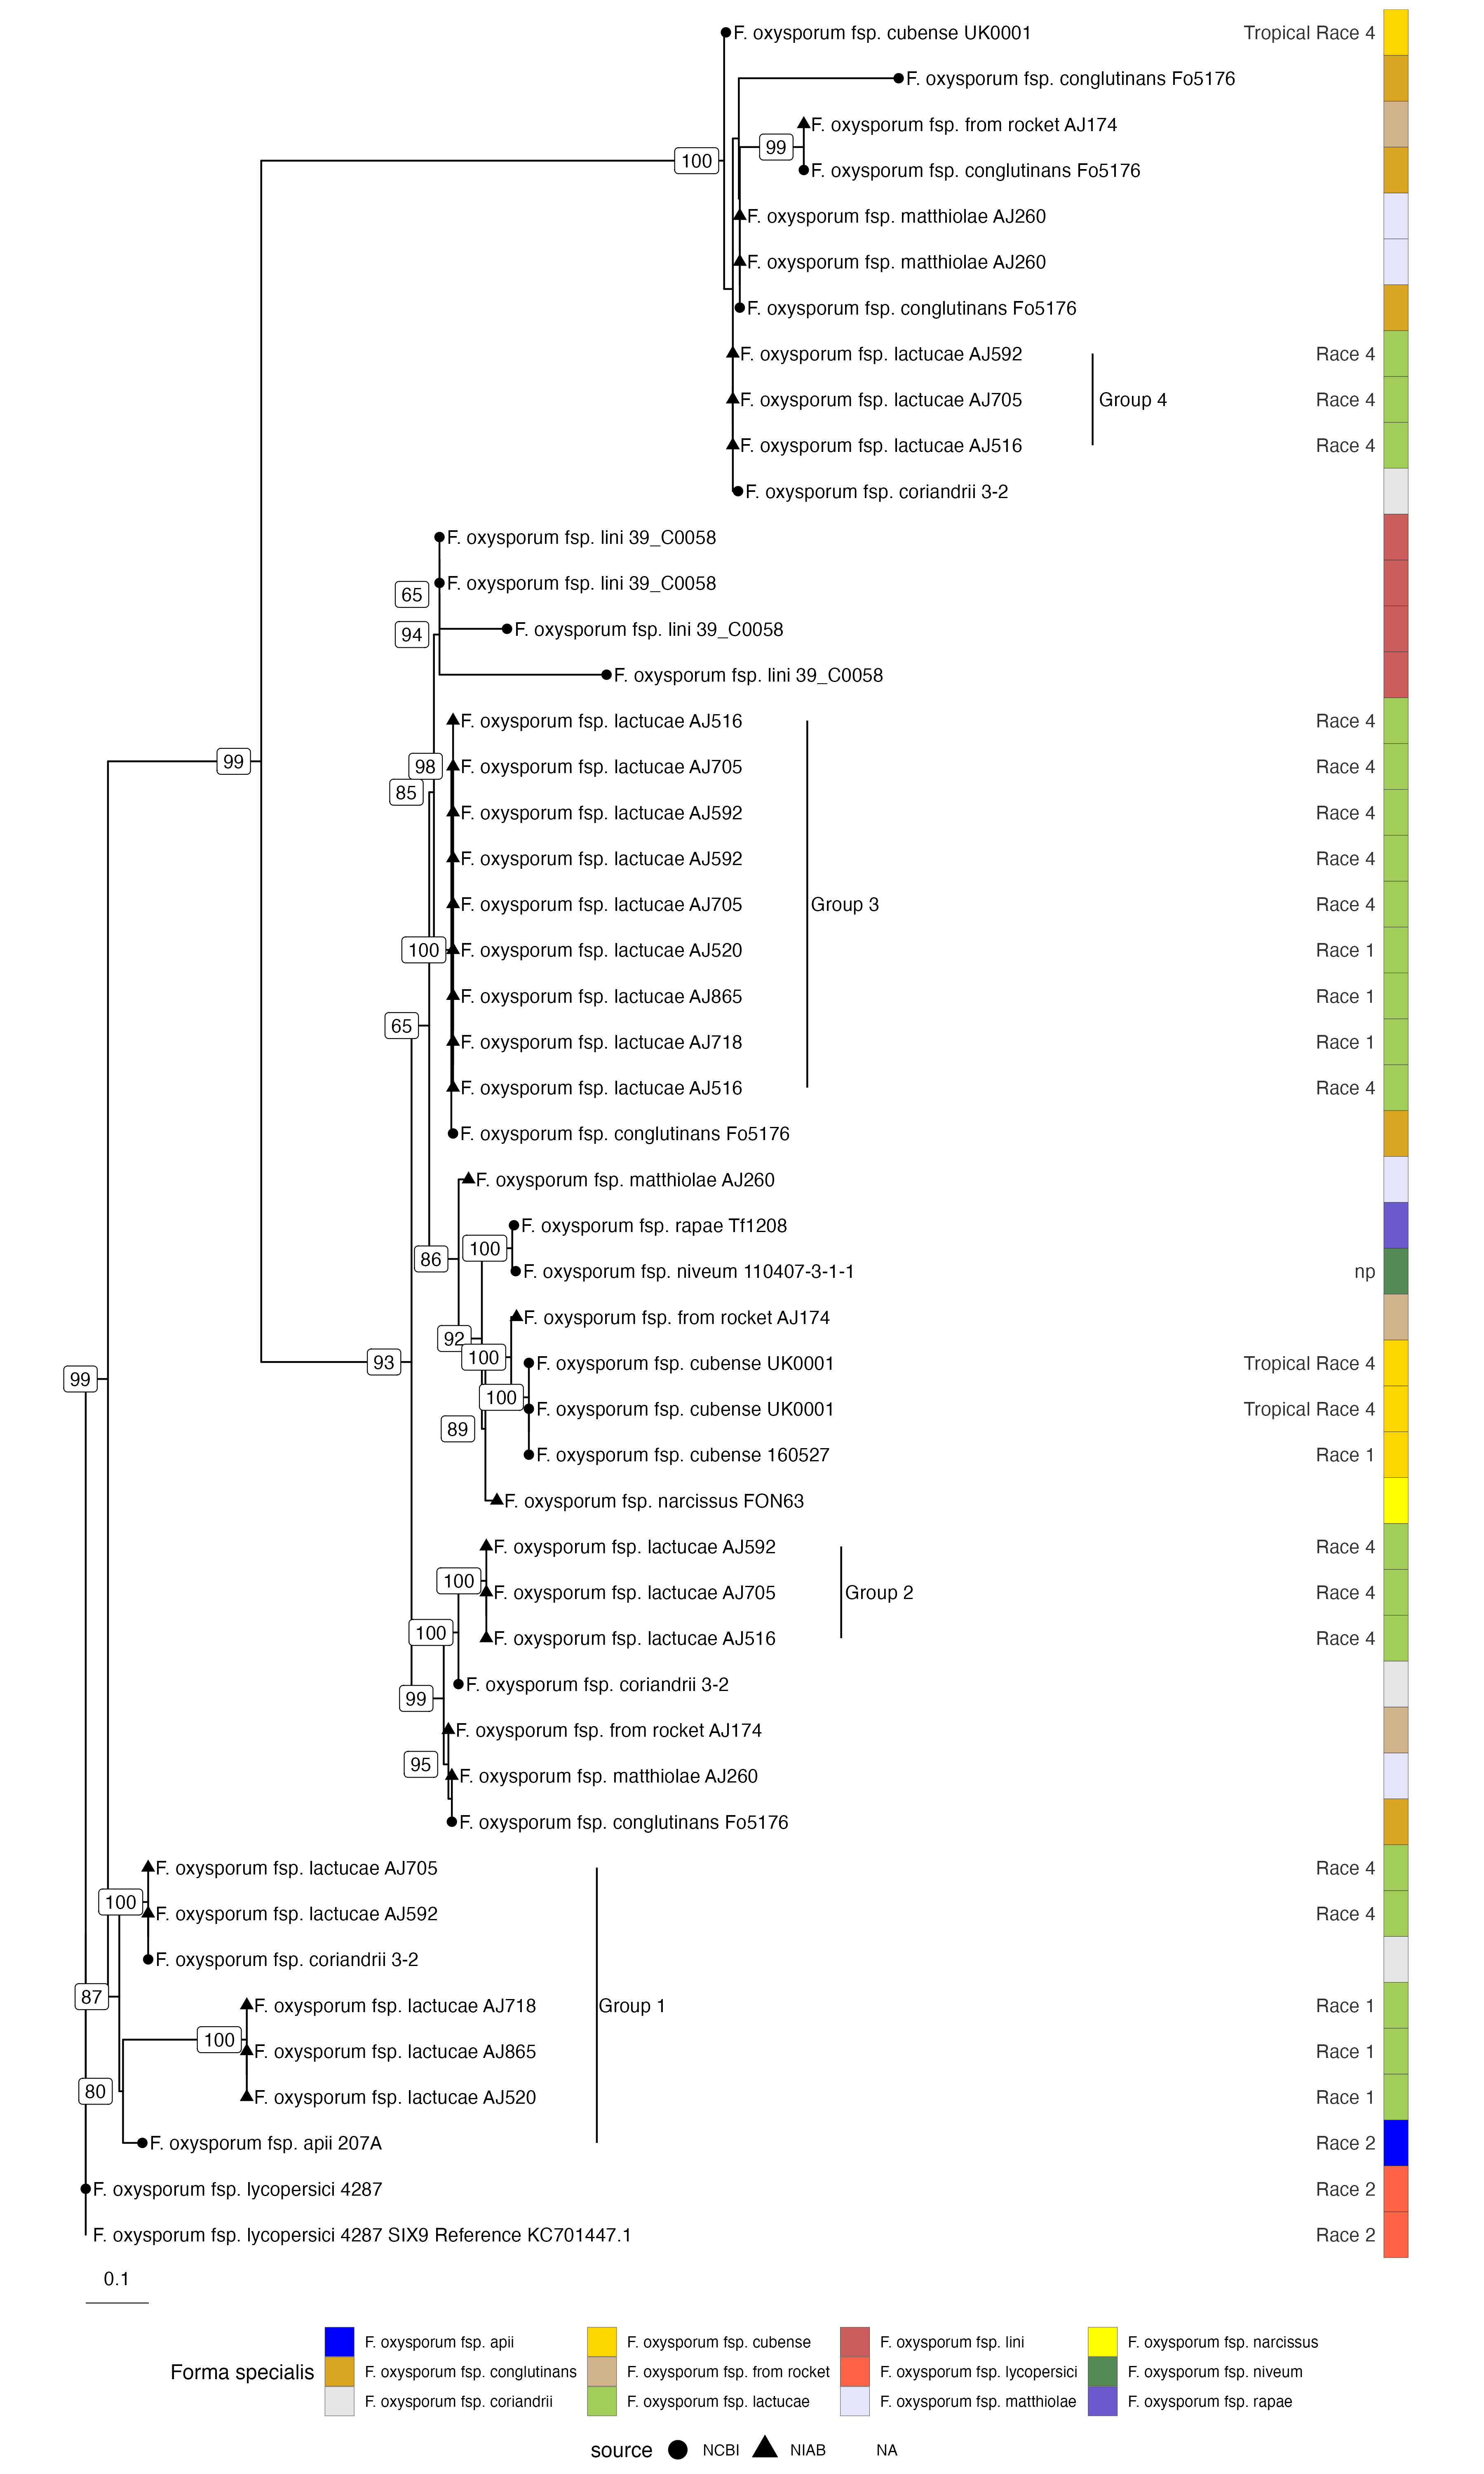
\includegraphics[width=12cm]{Figures/lactucaeSIX9tree.png}
    \captionsetup{width=\textwidth}
    \caption[Maximum likelihood phylogeny from alignment of \textit{SIX8} sequences from \acl{Fo} reveals differences in \acl{Fola} \textit{SIX9}.]{\textbf{Maximum likelihood phylogeny from alignment of \textit{SIX9} sequences from \acf{Fo} reveals differences in \acf{Fola} \textit{SIX9}.}  Branch length show expected number of substitutions per site. White boxes indicate bootstrap values from 1000 bootstrap replicates. IQ-TREE2 (v2.2.0.3) best model of substitution; TPM3+G4. The tree is rooted with the reference sequence \ac{Foly} \textit{SIX9} reference KC701447.1.1.}
    \label{fig:lactucae-six9}
\end{figure}

Each of the \ac{Fola} \ac{r4} isolates possessed one identical copy of \textit{SIX14}, two identical copies of the same \textit{SIX14} was identified in each \ac{Fola} \ac{r1} isolate (Group 1, Figure \ref{fig:lactucae-six14}). The \ac{Fola} \ac{r1} isolates possessed a third copy of \textit{SIX14} (Group 2, Figure \ref{fig:lactucae-six14}). The sequence variants of \textit{SIX14} across all \ac{Fola} isolates exhibited closer resemblance to each other than to homologues of \textit{SIX14} in other \ac{Fo} \acp{fsp}.

\begin{figure}[htp!]
    \centering
    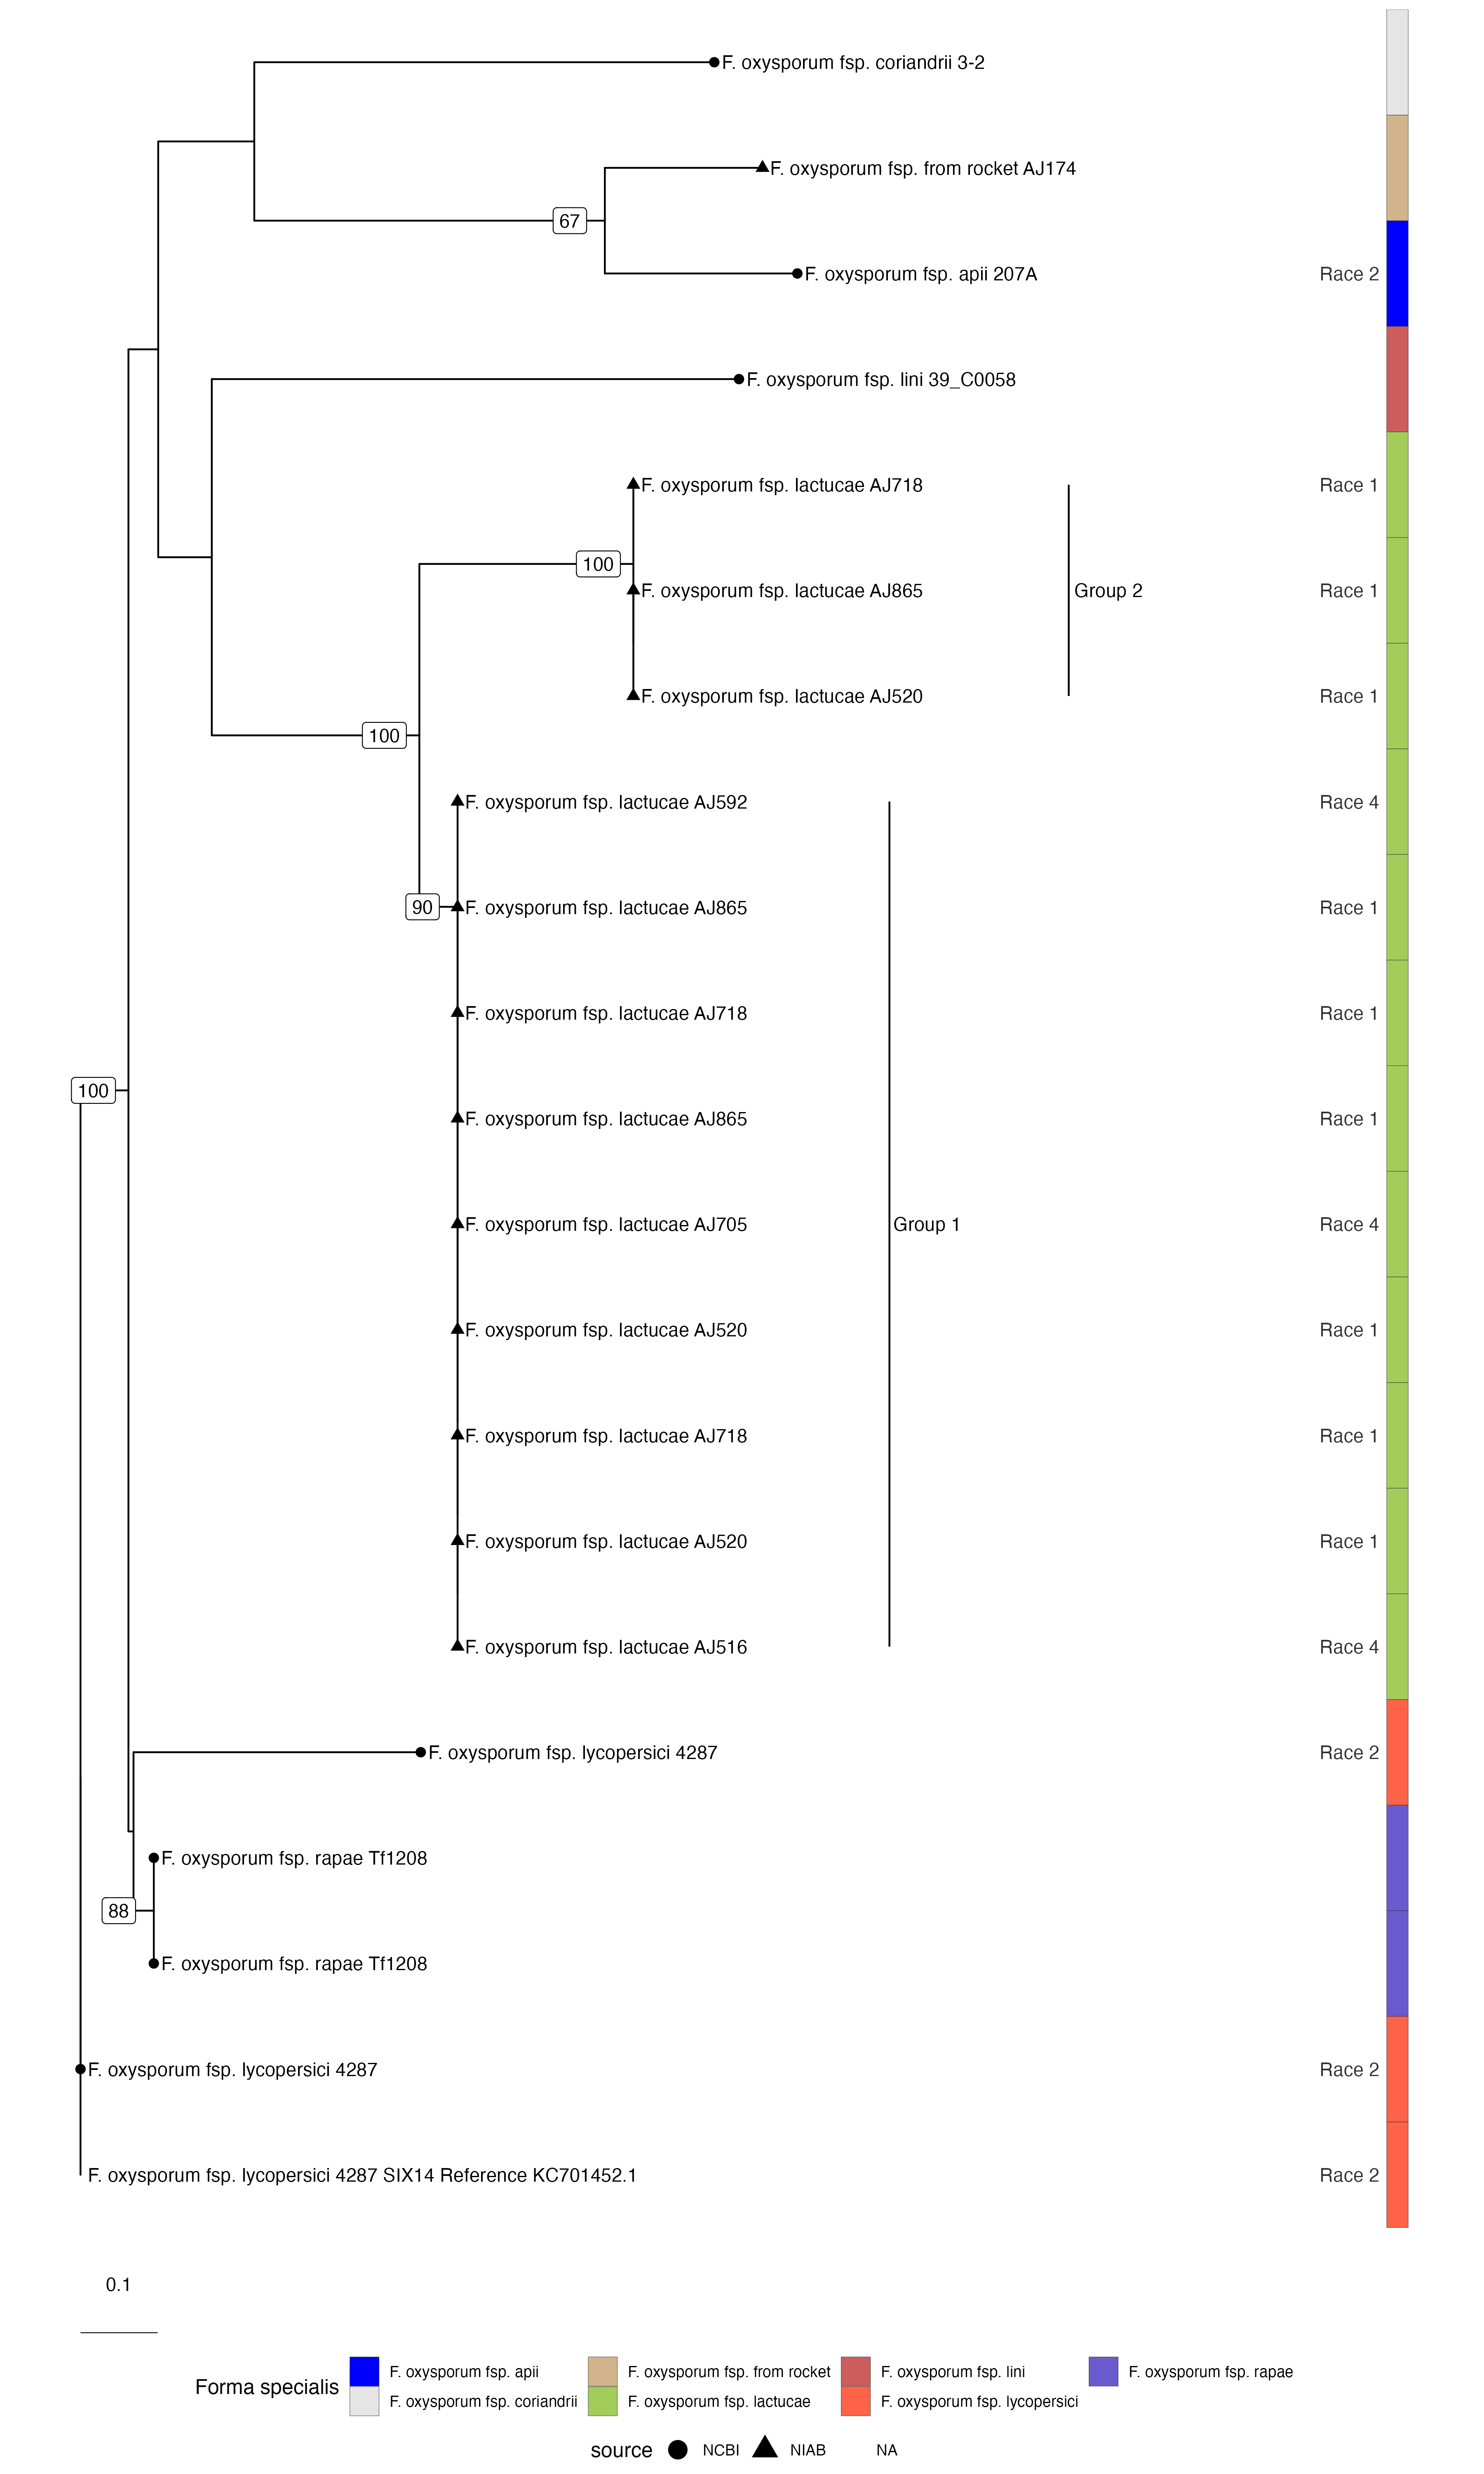
\includegraphics[width=12cm]{Figures/lactucaeSIX14tree.png}
    \captionsetup{width=\textwidth}
    \caption[Maximum likelihood phylogeny from alignment of \textit{SIX14} sequences from \acl{Fo} reveals differences in copy number of \textit{SIX14} between races of \acl{Fola}.]{\textbf{Maximum likelihood phylogeny from alignment of \textit{SIX14} sequences from \acf{Fo} reveals differences in copy number of \textit{SIX14} between races\acf{Fola}.}  Branch length show expected number of substitutions per site. White boxes indicate bootstrap values from 1000 bootstrap replicates. IQ-TREE2 (v2.2.0.3) best model of substitution; K2P+G4. The tree is rooted with the reference sequence \ac{Foly} \textit{SIX14} reference KC701452.1.}
    \label{fig:lactucae-six14}
\end{figure}

\subsection{Validation of \acl{maei} pipeline}
% - RNA seq of lactucae 
% - Ability of versions to predict effectors Table - Include FoEC.py first results?
% - Apii diagnostics 

\newpage
\section{Discussion}

Becuase isolates group based on fsp and race, we can be more confident we have identified effectors (compare to TEF phylo).

    Expections were: Foa and Foci: BUT...

    As \textcite{Henry2020} demonstrate, \ac{Foa} \ac{r3}, \ac{r4}, and \ac{Foci} (isolates 3-2 and GL306) have similar genomes and form a monophyletic group supported by our \ac{tef} phylogeny (Figure \ref{fig:TEF1aPhyloaMaei}). Further, \ac{Foa} \ac{r4} can also cause disease in coriander (\textit{Coriandrum sativum}), the host of \ac{Foci} \parencite{Epstein2022}. 

limitations of \% identity thresholds. 
 - Arbitrary! 
 - Some of these core CECs were also found in the non-pathogens, could be that the CE sequences is different which allows for pathogneicty, could also be that the effector is not involved in virulence!

PCA ffector clusters?

\subsection{}{Segmental duplication and the evolution of effectors}

van Westerhoven \et (2023) investigated the effects of segmental duplications on effector repertoires.  Though previously reported by van Dam \et (2016), the authors provide a more comprehensive effector gene repertoire for \ac{Focub} and demonstrate that effector repertoires were variable among the strains. The study found that 336 out of 669 predicted effector genes in \ac{Focub4} strain II5 evolved via segmental duplications. Notably, the effector SIX1, which is essential for full virulence to banana, was found to be part of a segmental duplication. This supports van Westerhoven \et (2023) argument and suggests that segmental duplications are involved in the evolution and diversification of effector genes in \ac{Focub}, which in turn influence the pathogenicity and virulence of \textit{Fusarium} strains.

Though we know that cytoplasmic fungal effectors are secreted into plant host cells, the mechanism by which fungal pathogens deliver effector proteins into plant cells remains poorly understood. Recently, \textcite{Oliveira-Garcia2023, Wang2023} have provided evidence for the uptake of cytoplasmic effectors from \textit{Magnaporthe oryzae} and \textit{Phytophthora infestans} into host \textit{Oryza sativa} or \textit{Nicotiana benthamiana} cells, respectively, through clathrin-mediated endocytosis (CME).  

\textcolor{red}{[ALSO, IF YOU USE EFFECTORS AS A TARGET, THEY ARE PRONE TO HIGH AMOUNTS OF EVOLUTIONARY PRESSURE, AND MAY MUTATE RENDERDING DIAGNOSTICS USELESS - YOU THEREFORE NEED A MEANS OF CONSISTENTLY INDENTIFYING NEW TARGETS...]}

Using structure to predict candidates?